\section{Transformers}
\title{Transformers}  

\begin{frame}[plain]
    \titlepage
\end{frame}

%%%%%%%%%%%%%%%%%%%%%%%%%%%%%%%%%%%%%%%%%%%%%%%%%%%%%%%%%%%%%
%% Transformer definition %%
%%%%%%%%%%%%%%%%%%%%%%%%%%%%%%%%%%%%%%%%%%%%%%%%%%%%%%%%%%%%%
\begin{frame}
	\frametitle{Transformer definition}
    \begin{columns}
		\begin{column}{0.65\textwidth}
            \begin{varblock}{Transformer}
                A transformer is a static device that transfers electrical energy between two or more circuits through electromagnetic induction. It converts the AC voltage levels between inputs and outputs.   
            \end{varblock}
            \begin{itemize}
                \item<2-> While a transformer is sometimes called a ``static~machine'', it does not meet the formal definition of an electrical machine (compare first chapter).
                \item<3-> However, transformers share some working principles with electrical machines and are also often used as components of electrical power systems including drives.
            \end{itemize}
		\end{column}
        \hfill
		\begin{column}{0.35\textwidth}
			\onslide<1->
			\begin{figure}
				\centering
				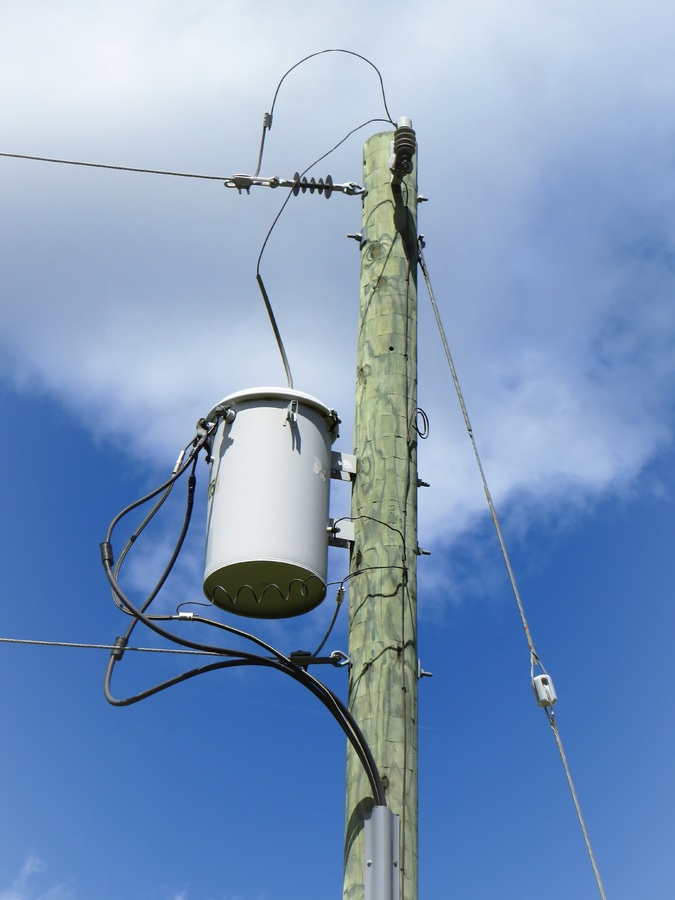
\includegraphics[width=0.75\textwidth]{fig/lec04/Transformer_rural_pole.jpg}
				\caption{Transformer integrated at a utility pole (source: \href{https://pxhere.com/en/photo/795672}{pxhere.com}, public domain)}
			\end{figure}
		\end{column}
		\end{columns}
\end{frame}


%%%%%%%%%%%%%%%%%%%%%%%%%%%%%%%%%%%%%%%%%%%%%%%%%%%%%%%%%%%%%
%% Need of Transformers %%
%%%%%%%%%%%%%%%%%%%%%%%%%%%%%%%%%%%%%%%%%%%%%%%%%%%%%%%%%%%%%
\begin{frame}
	\frametitle{Function and example use of transformers}
    \begin{columns}
		\begin{column}{0.45\textwidth}
            \begin{itemize}
              \item Voltage level adjustment: Can help to make increase or decrease voltage level(\textbf{step-up} for increase and \textbf{step-down} for decreasing). 
              \item Electrical isolation: Provides galvanic isolation between circuits, enhancing safety and reducing noise.
              \item Impedance matching: Helps in matching impedance between different electrical devices or systems to maximize power transfer and minimize losses (\textbf{Maximum power transfer theorem!})
              \item Load sharing:  Multiple transformers can share load in parallel operation, improving system reliability and flexibility.
            \end{itemize}
		\end{column}
        \hfill
		\begin{column}{0.525\textwidth}
        \begin{itemize}
          \item Example need of transformers- power systems
          \begin{itemize}
            \item The wires in power systems have resistance --> $I^2R$/Joule losses eminent
            \item Ohm's law (V=IR), increase "V" reduce "I".  
            \item So, at increased voltage, the same power can be delivered by a high-voltage transmission line in reduced current but higher efficiency. 
          \end{itemize}
			\begin{figure}
				\centering
				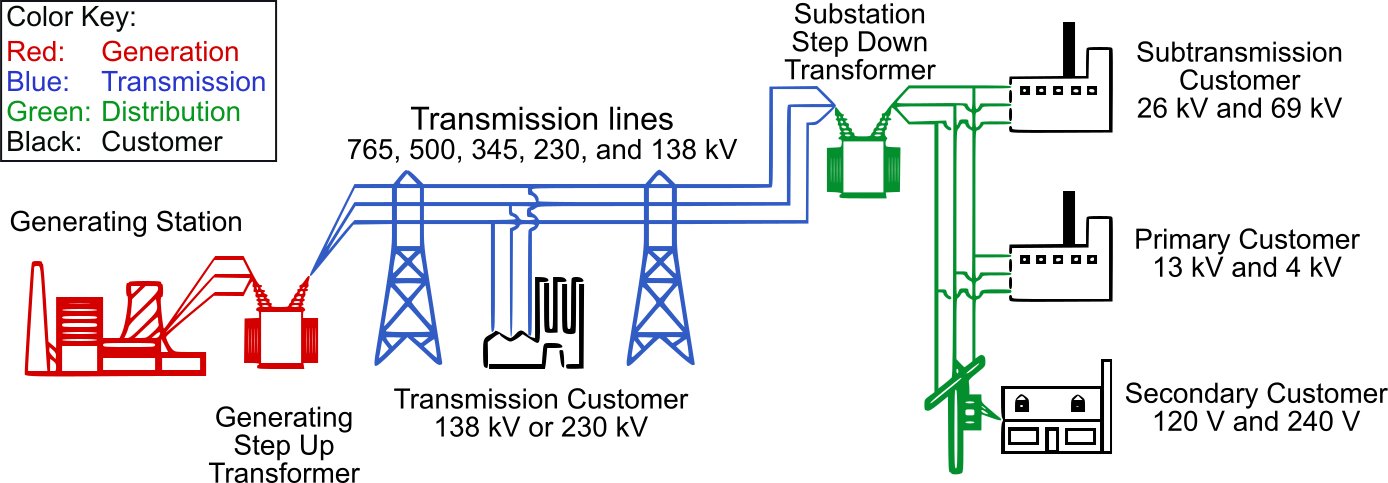
\includegraphics[width=0.75\textwidth]{fig/lec04/Electricity_grid_simple.png}
				\caption{Diagram of electric grid (source: \href{https://commons.wikimedia.org/wiki/File:Electricity_grid_simple-_North_America.svg}{United States Department of Energy, SVG version by User:J JMesserly, Public domain, via Wikimedia Commons}, public domain)}
			\end{figure}
        \end{itemize}

		\end{column}
		\end{columns}
\end{frame}


%%%%%%%%%%%%%%%%%%%%%%%%%%%%%%%%%%%%%%%%%%%%%%%%%%%%%%%%%%%%%
%% Examples of transformers %%
%%%%%%%%%%%%%%%%%%%%%%%%%%%%%%%%%%%%%%%%%%%%%%%%%%%%%%%%%%%%%
\begin{frame}
	\frametitle{Examples of transformers}
	\begin{figure}
		\centering
		\begin{subfigure}[b]{0.49\textwidth}
			\centering
			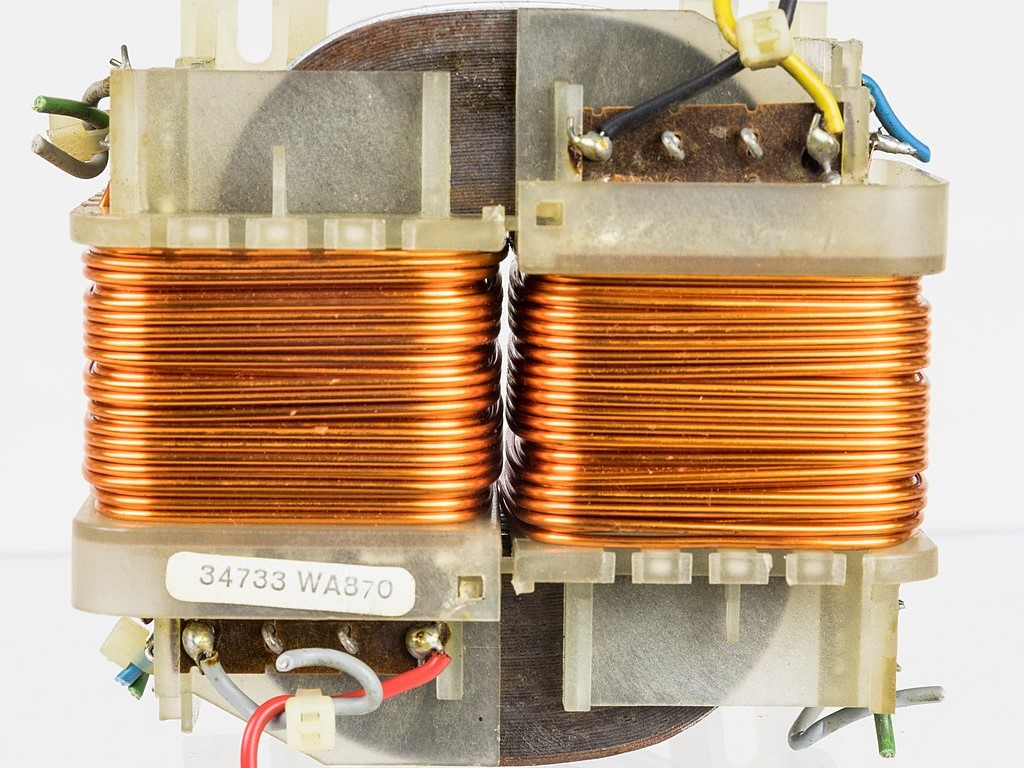
\includegraphics[width=0.45\textwidth]{fig/lec04/Power_supply_transformer.jpg}
			\caption{Power supply transformer (source: \href{https://commons.wikimedia.org/wiki/File:Philips_N4422_-_power_supply_transformer-2098.jpg}{Wikimedia Commons}, R.~Spekking, \href{https://creativecommons.org/licenses/by-sa/4.0/deed}{CC BY-SA 4.0})}
		\end{subfigure}
		\hfill
		\begin{subfigure}[b]{0.49\textwidth}
			\centering
			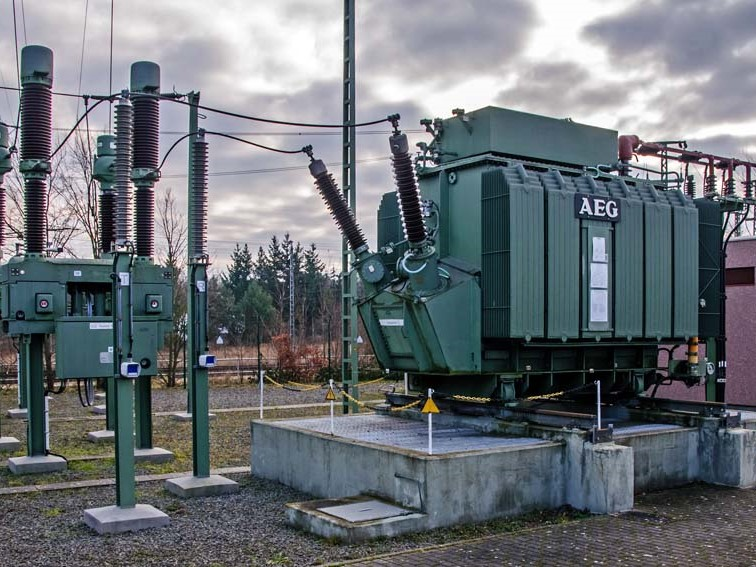
\includegraphics[width=0.45\textwidth]{fig/lec04/Single_phase_transformer.jpg}
			\caption{Single-phase transformer (source: \href{https://commons.wikimedia.org/wiki/File:DB_Unterwerk_Güsen,_Trafo_p.jpg}{Wikimedia Commons}, Georg, \href{https://creativecommons.org/licenses/by-sa/4.0/deed.en}{CC BY-SA 4.0})}
		\end{subfigure}
		\\
		\begin{subfigure}[b]{0.49\textwidth}
			\centering
			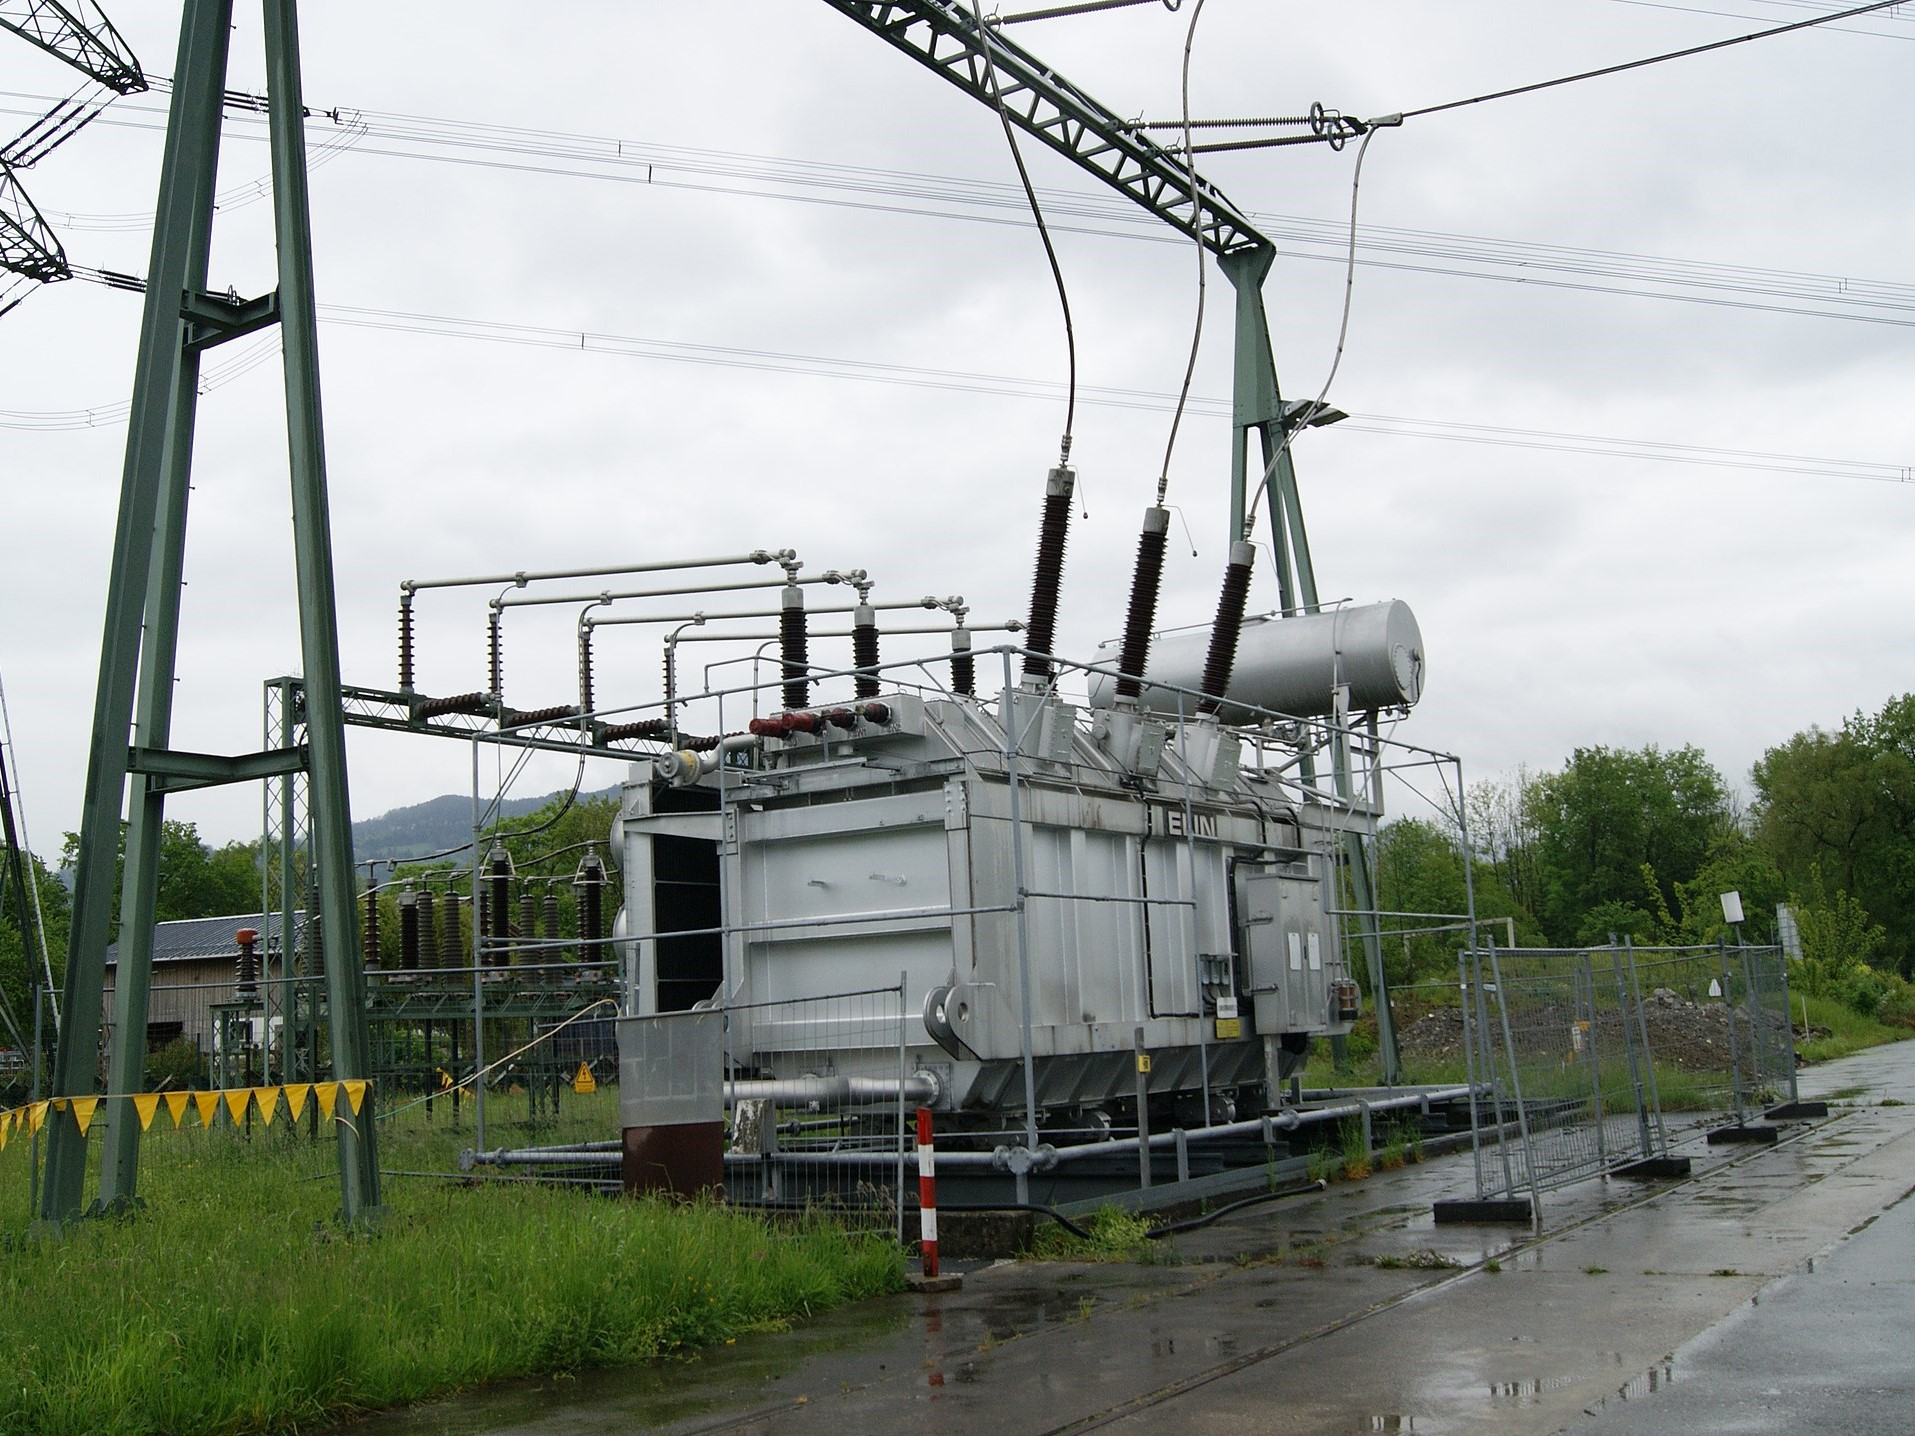
\includegraphics[width=0.45\textwidth]{fig/lec04/Three_phase_transformer.jpg}
			\caption{Three-phase transformer (source: \href{https://commons.wikimedia.org/wiki/File:Dornbirn-Umspannwerk_Werben-110kV_FS6-Anlage_Trafo_Elin_220-110kV-01ASD.jpg}{Wikimedia Commons}, Asurnipal, \href{https://creativecommons.org/licenses/by-sa/4.0/deed.en}{CC BY-SA 4.0})}
		\end{subfigure}
		\hfill
		\begin{subfigure}[b]{0.49\textwidth}
			\centering
			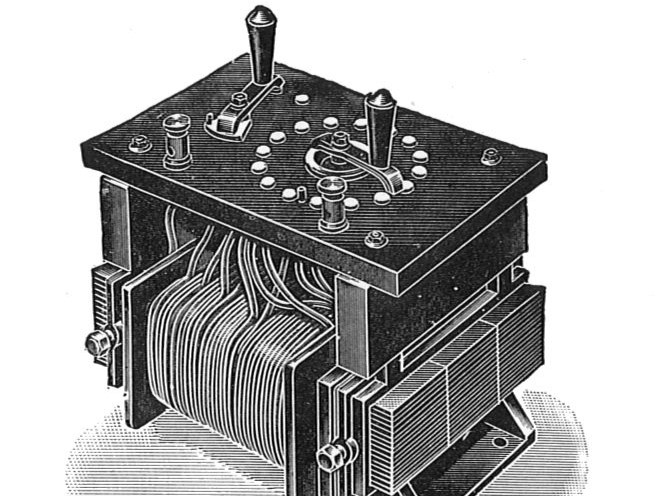
\includegraphics[width=0.45\textwidth]{fig/lec04/Tapped_transformer.jpg}
			\caption{Variable tapped transformer (source: \href{https://commons.wikimedia.org/wiki/File:Variable-tap_regulating_transformer_(Rankin_Kennedy,_Electrical_Installations,_Vol_II,_1909).jpg}{Wikimedia Commons}, public domain)}
		\end{subfigure}
		\caption*{Examples of transformers} 
        \label{fig:examples_transformers}
	\end{figure}
\end{frame}

%%%%%%%%%%%%%%%%%%%%%%%%%%%%%%%%%%%%%%%%%%%%%%%%%%%%%%%%%%%%%
%% Types of Transformers %%
%%%%%%%%%%%%%%%%%%%%%%%%%%%%%%%%%%%%%%%%%%%%%%%%%%%%%%%%%%%%%
\begin{frame}
	\frametitle{Types of transformers and working principle}
    \begin{columns}
     \begin{column}{0.55\textwidth}
      \begin{itemize}
          \item Based on voltage transformation- step up and step down.
          \item Based on number of phases- single phase, three phase, multi phase. 
          \item Based on usage- power transformers typically used as generation transformer, transmission transformer, distribution transformers, current transformers (CT), voltage transformers (PT), isolation transformers, etc. 
          \item Based on core medium- air core, iron/steel core, ferrite core, and nanocrystalline core.
          \item Based on construction- core type and shell type. 
      \end{itemize}      
      \end{column}
      \begin{column}{0.45\textwidth}
      			\onslide<1->
			\begin{figure}
				\centering
				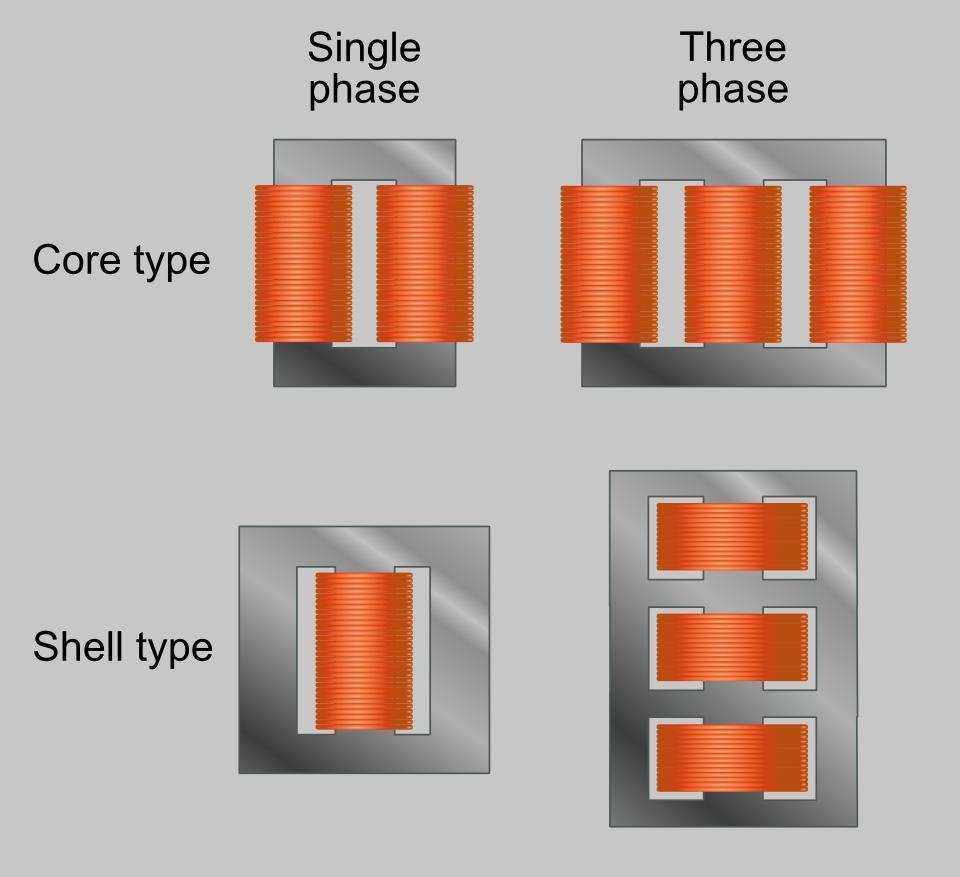
\includegraphics[height=0.575\textheight]{fig/lec04/Transformer_winding_formats.jpg}
                \caption{Transformer winding formats (source: \href{https://commons.wikimedia.org/wiki/File:Transformer_winding_formats.jpg}{Wikimedia Commons}, CC BY-SA 3.0)}
			\end{figure}
      \end{column}
    \end{columns}   
\end{frame}

%%%%%%%%%%%%%%%%%%%%%%%%%%%%%%%%%%%%%%%%%%%%%%%%%%%%%%%%%%%%%
%% Basic working principle of transformers %%
%%%%%%%%%%%%%%%%%%%%%%%%%%%%%%%%%%%%%%%%%%%%%%%%%%%%%%%%%%%%%
\begin{frame}
	\frametitle{Basic working principle- Faraday's Law of Electromagnetic Induction}
    \begin{columns}
     \begin{column}{0.45\textwidth}
      \begin{itemize}
        \item A changing magnetic flux in the primary coil induces an electromotive force (EMF) in the secondary coil.
        \item Mathematical expression: $\text{EMF} \propto \frac{d\psi}{dt}$, where $\psi$ is the magnetic flux linkage through the core and $\frac{d\psi}{dt}$ is the rate of change of magnetic flux.
        \item An alternating current in the \textbf{primary winding} produces a time-varying magnetic field. This magnetic field links with the \textbf{secondary winding} through a magnetic core. The changing flux induces a voltage in the secondary winding.
      \end{itemize}
      \end{column}
      \begin{column}{0.45\textwidth}
			\onslide<1->
			\begin{figure}
				\centering
				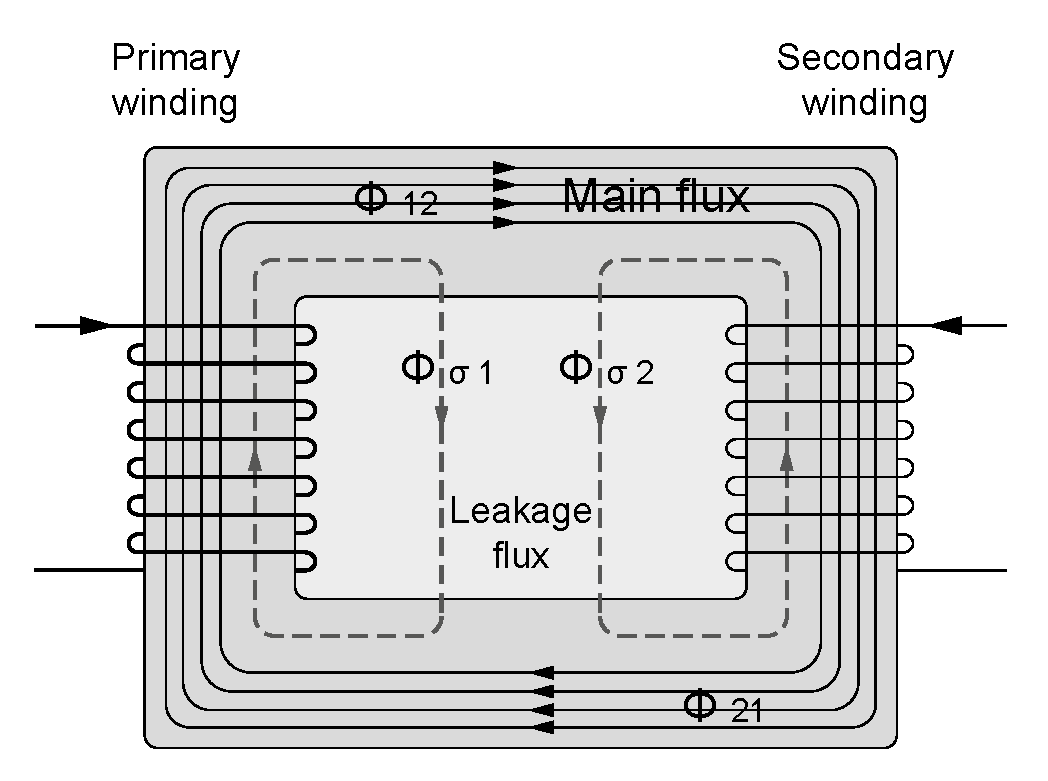
\includegraphics[height=0.575\textheight]{fig/lec04/trans_flux.pdf}
                \caption{Transformer flux linkage for working principle (source: \href{https://upload.wikimedia.org/wikipedia/commons/6/63/Transformer_Flux.svg}{Wikimedia Commons}, Fred the Oyster, CC BY-SA 4.0)}
			\end{figure}
      \end{column}
    \end{columns}  
\end{frame}


%%%%%%%%%%%%%%%%%%%%%%%%%%%%%%%%%%%%%%%%%%%%%%%%%%%%%%%%%%%%%
%% Dot convention %%
%%%%%%%%%%%%%%%%%%%%%%%%%%%%%%%%%%%%%%%%%%%%%%%%%%%%%%%%%%%%%
\begin{frame}
	\frametitle{Dot convention in transformers}
    \begin{columns}
     \begin{column}{0.75\textwidth}
      \begin{itemize}
        \item "Dot convention" or "Dot notation"- a method of indicating the relative polarity or phase relationship between the primary and secondary windings.
        \item \textbf{Purpose}: helps engineers and technicians understand the polarity of transformer windings.
        \item Dots mentioned-- polarity important, else, does not matter. 
        \item If current flows into the dotted terminal of one coil, the induced mutual voltage in the other coil will be positive at its dotted terminal. Conversely, if current flows out of the dotted terminal, the induced voltage will be negative at the dotted terminal.
        \item The polarity of the mutually induced voltage depends on the direction of current relative to the dot: current entering the dotted end of one winding results in a positive polarity at the dot of the coupled winding, while current leaving the dotted terminal results in a negative polarity at the other dot.
      \end{itemize}
      \end{column}
      \begin{column}{0.25\textwidth}
			\onslide<1->
			\begin{figure}
				\centering
				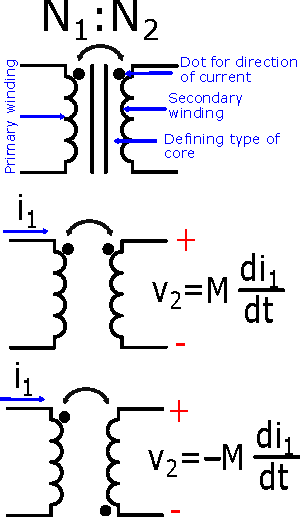
\includegraphics[height=0.575\textheight]{fig/lec04/dot_convention.pdf}
                \caption{Dot convention in transformer}
			\end{figure}
      \end{column}
    \end{columns}  
\end{frame}

%%%%%%%%%%%%%%%%%%%%%%%%%%%%%%%%%%%%%%%%%%%%%%%%%%%%%%%%%%%%%
%% Electromagnetic modeling of the single-phase transformer %%
%%%%%%%%%%%%%%%%%%%%%%%%%%%%%%%%%%%%%%%%%%%%%%%%%%%%%%%%%%%%%
\begin{frame}
	\frametitle{Electromagnetic modeling of the single-phase transformer}
    \begin{columns}
		\begin{column}{0.45\textwidth}
            Recap from \eqref{eq:flux_linkage_matrix_transformer}: for some given current $\bm{i}$, the flux linkages $\bm{\psi}$ in the transformer windings are
			\begin{equation*}
				\bm{\psi} = \begin{bmatrix} \psi_1 \\ \psi_2 \end{bmatrix} = \begin{bmatrix} L_1 & M \\ M & L_2 \end{bmatrix} \begin{bmatrix} i_1 \\ i_2 \end{bmatrix} = \bm{L}\bm{i}
			\end{equation*}
			where $L_1$ and $L_2$ are the self-inductances of the primary and secondary winding, respectively, and $M$ is the mutual inductance.
			\\[1em] \pause
			Note: The above equation is an algebraic relation, that is, it is valid for any time instant $t$ and applies to both AC and DC excitation of the transformer. 
		\end{column}
        \hfill
		\begin{column}{0.525\textwidth}
			\onslide<1->
			\begin{figure}
				\centering
				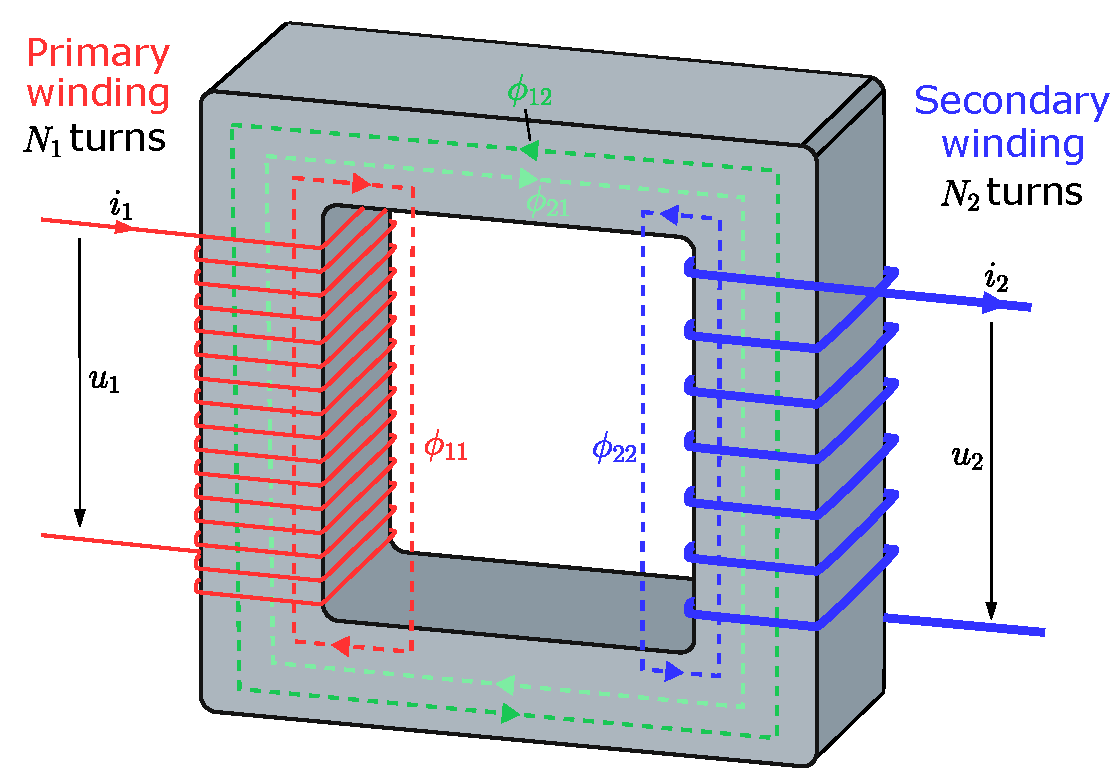
\includegraphics[height=0.575\textheight]{fig/lec02/Transformer3d_col3.pdf}
			\end{figure}
		\end{column}
		\end{columns}
\end{frame}

%%%%%%%%%%%%%%%%%%%%%%%%%%%%%%%%%%%%%%%%%%%%%%%%%%%%%%%%%%%%%
%% Dynamic modeling of the single-phase transformer %%
%%%%%%%%%%%%%%%%%%%%%%%%%%%%%%%%%%%%%%%%%%%%%%%%%%%%%%%%%%%%%
\begin{frame}
	\frametitle{Dynamic modeling of the single-phase transformer}
		The dynamic transformer behavior can be represented by the ECD in \figref{fig:General_transformer_ECD}, which also considers the internal resistances of the windings. Applying Faraday's law, the resulting differential equations are:
		\begin{align}
			u_1(t) = R_1 i_1(t) + \frac{\mathrm{d}\psi_1(t)}{\mathrm{d}t}, \qquad u_2(t) = R_2 i_2(t) + \frac{\mathrm{d}\psi_2(t)}{\mathrm{d}t}. \label{eq:transformer_differential_equations}
		\end{align} \pause
		Inserting \eqref{eq:flux_linkage_matrix_transformer} delivers:
		\begin{align}
			u_1(t) = R_1 i_1(t) + L_1 \frac{\mathrm{d}i_1(t)}{\mathrm{d}t} + M \frac{\mathrm{d}i_2(t)}{\mathrm{d}t}, \qquad
			u_2(t) = R_2 i_2(t) + L_2 \frac{\mathrm{d}i_2(t)}{\mathrm{d}t} + M \frac{\mathrm{d}i_1(t)}{\mathrm{d}t}. \label{eq:transformer_differential_equations_2}
		\end{align}
\begin{figure}
\onslide<1->
\begin{columns}
	\begin{column}{0.55\textwidth}
            \centering
            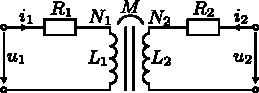
\includegraphics[width=0.8\textwidth]{fig/lec04/General_transformer_ECD.pdf}
    \end{column}
    \begin{column}{0.45\textwidth}
        \caption{\raggedright General equivalent circuit diagram (ECD) of a transformer (note: that both ports of the transformer are denoted in the load convention reference frame which is an arbitrary representation decision).}
		\label{fig:General_transformer_ECD}
    \end{column}
\end{columns}
\end{figure}
\end{frame}

%%%%%%%%%%%%%%%%%%%%%%%%%%%%%%%%%%%%%%%%%%%%%%%%%%%%%%%%%%%%%
%% Dynamic modeling of the single-phase transformer (cont.) %%
%%%%%%%%%%%%%%%%%%%%%%%%%%%%%%%%%%%%%%%%%%%%%%%%%%%%%%%%%%%%%
\begin{frame}
	\frametitle{Dynamic modeling of the single-phase transformer (cont.)}
		The model \eqref{eq:transformer_differential_equations_2} can be represented by the T-type ECD in \figref{fig:Transformer_T_ECD}. It may be noted that $L_1-M$ and $L_2-M$ can have negative values due to the model representation. 
		\\[1em] \pause
		By rearranging \eqref{eq:transformer_differential_equations_2}, we can also write the dynamic transformer model in vector-matrix form:
		\begin{equation}
			\begin{bmatrix}	u_1(t)\\u_2(t) \end{bmatrix} = \bm{u}(t) = \begin{bmatrix} R_1 & 0 \\ 0 & R_2 \end{bmatrix} \begin{bmatrix} i_1(t)\\i_2(t) \end{bmatrix} + \begin{bmatrix} L_1 & M \\ M & L_2 \end{bmatrix} \frac{\mathrm{d}}{\mathrm{d}t} \begin{bmatrix} i_1(t)\\i_2(t) \end{bmatrix} = \bm{R}\bm{i}(t) + \bm{L}\frac{\mathrm{d}}{\mathrm{d}t}\bm{i}(t).  
			\label{eq:transformer_differential_equations_matrix_form}
		\end{equation}
\begin{figure}
\begin{columns}
	\onslide<1->
	\begin{column}{0.55\textwidth}
            \centering
            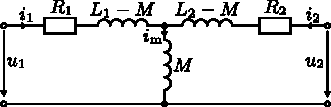
\includegraphics[width=0.9\textwidth]{fig/lec04/Transformer_T_ECD.pdf}
    \end{column}
    \begin{column}{0.45\textwidth}
        \caption{\raggedright T-type ECD of a transformer (note that the model \eqref{eq:transformer_differential_equations_matrix_form} assumes linear time-invariant (LTI) behavior, which among other effects neglects magnetic saturation).}
		\label{fig:Transformer_T_ECD}
    \end{column}
\end{columns}
\end{figure}
\end{frame}

%%%%%%%%%%%%%%%%%%%%%%%%%%%%%%%%%%%%%%%%%%%%%%%%%%%%%%%%%%%%%
%% Dynamic modeling of the single-phase transformer (cont.) %%
%%%%%%%%%%%%%%%%%%%%%%%%%%%%%%%%%%%%%%%%%%%%%%%%%%%%%%%%%%%%%
\begin{frame}
	\frametitle{Dynamic modeling of the single-phase transformer (cont.)}
		Rearranging \eqref{eq:transformer_differential_equations_matrix_form} gives the state-space representation of the transformer model
		\begin{equation}
			\frac{\mathrm{d}}{\mathrm{d}t}\bm{i}(t) = \bm{L}^{-1}\left(\bm{u}(t)-\bm{R}\bm{i}(t) \right)
			\label{eq:transformer_state_space_01}
		\end{equation}
		with
		$$ \renewcommand*{\arraystretch}{1.3} \bm{L}^{-1} = \frac{1}{L_1L_2 - M^2} \begin{bmatrix} L_2 & -M \\ -M & L_1 \end{bmatrix} = \frac{1}{\sigma} \begin{bmatrix} \frac{1}{L_1} &  \frac{-M}{L_1 L_2} \\ \frac{-M}{L_1 L_2} & \frac{1}{L_2} \end{bmatrix}.$$
		\pause
		Above, $\sigma$ is the leakage coefficient defined as (compare also \eqref{eq:coupling_coefficient})
		\begin{equation}
			\sigma = \frac{L_1 L_2 -M^2}{L_1 L_2 } = 1 - \frac{M^2}{ L_1 L_2} = 1 - k^2 .
			\label{eq:leakage_coefficient}
		\end{equation}
		\pause
		Finally, the state-space representation of the transformer model (with the currents as states) is
		\begin{equation}
			\renewcommand*{\arraystretch}{1.3} 
			\frac{\mathrm{d}}{\mathrm{d}t}\bm{i}(t) = \begin{bmatrix} -\frac{R_1}{\sigma L_1} & \frac{R_2 M}{\sigma L_1 L_2} \\ \frac{R_1 M}{\sigma L_1 L_2} & -\frac{R_2}{\sigma L_2} \end{bmatrix} \bm{i}(t) + \begin{bmatrix} \frac{1}{\sigma L_1} & -\frac{M}{\sigma L_1 L_2} \\ -\frac{M}{\sigma L_1 L_2} & \frac{1}{\sigma L_2} \end{bmatrix} \bm{u}(t) = \bm{A} \bm{i}(t) + \bm{B} \bm{u}(t) .	 
			\label{eq:transformer_state_space_02}
		\end{equation}
\end{frame}

%%%%%%%%%%%%%%%%%%%%%%%%%%%%%%%%%%%%%%%%%%%%%%%%%%%%%%%%%%%%%
%% Steady-state of the single-phase transformer %%
%%%%%%%%%%%%%%%%%%%%%%%%%%%%%%%%%%%%%%%%%%%%%%%%%%%%%%%%%%%%%
\begin{frame}
	\frametitle{Steady-state modeling of the single-phase transformer}
		Assuming that the transformer operates in steady state and that all quantities are sinusoidal, the state-space model \eqref{eq:transformer_state_space_02} can be simplified and represented by complex phasors:
			$$x(t) = \hat{x} \cos(\omega_\mathrm{el} t+ \varphi_{\mathrm{x}}) = \mathrm{Re}\left\{\hat{x} e^{\iu (\omega_\mathrm{el} t + \varphi_{\mathrm{x}})}\right\}= \mathrm{Re}\left\{\underline{X} e^{\iu \omega_\mathrm{el} t}\right\}.$$
			\pause
		From \eqref{eq:transformer_differential_equations_matrix_form} we receive
		\begin{align}
			\bm{\underline{U}} = \begin{bmatrix} \underline{U}_1 \\ \underline{U}_2 \end{bmatrix} = \bm{R}\bm{\underline{I}} + \iu \omega_\mathrm{el} \bm{L}\bm{\underline{I}} = \bm{\underline{Z}}\, \bm{\underline{I} } = \begin{bmatrix} R_1 + \iu \omega_\mathrm{el} L_1 & \iu \omega_\mathrm{el} M \\ \iu \omega_\mathrm{el} M & R_2 + \iu \omega_\mathrm{el} L_2 \end{bmatrix} \begin{bmatrix} \underline{I}_1 \\ \underline{I}_2 \end{bmatrix}.
			\label{eq:transformer_steady_state_voltage_response}
		\end{align}
		\pause
		For some given $\bm{\underline{U}}$ we can calculate the current phasor $\bm{\underline{I}}$ (i.e., the steady-state current response) by solving:
		\begin{align}
			\renewcommand*{\arraystretch}{1.3} 
			\bm{\underline{I}} = \bm{\underline{Z}}^{-1} \bm{\underline{U}} .
			\label{eq:transformer_steady_state_current_response}
		\end{align}
		\pause
		Alternative scenarios can be also considered, e.g., defining $\underline{U}_1$ (input voltage) and $\underline{I}_2$ (load current) as given and solving for $\underline{I}_1$ and $\underline{U}_2$ by rearranging \eqref{eq:transformer_steady_state_voltage_response}. 
\end{frame}

%%%%%%%%%%%%%%%%%%%%%%%%%%%%%%%%%%%%%%%%%%%%%%%%%%%%%%%%%%%%%
%% Steady-state of the single-phase transformer (cont.) %%
%%%%%%%%%%%%%%%%%%%%%%%%%%%%%%%%%%%%%%%%%%%%%%%%%%%%%%%%%%%%%
\begin{frame}
	\frametitle{Steady-state modeling of the single-phase transformer (cont.)}
		Assuming that the transformer is not loaded ($I_2 = 0$) and that it is lossless ($R_1 = 0$), \eqref{eq:transformer_steady_state_voltage_response} simplifies to
		\begin{equation}
			\begin{bmatrix} \underline{U}_1 \\ \underline{U}_2 \end{bmatrix} = \begin{bmatrix} \iu \omega_\mathrm{el} L_1  \\ \iu \omega_\mathrm{el} M  \end{bmatrix} \underline{I}_1.
		\end{equation} \pause
		The voltage transformation ratio in this case results in
		\begin{equation}
			\frac{U_1}{U_2} = \frac{\iu \omega_{\mathrm{el}} L_1 I_1}{\iu \omega_{\mathrm{el}} M I_1}  = \frac{L_1}{M}.
		\end{equation}
		\pause
		Assuming further that the transformer is leakage-free ($L_{1,\sigma}=0$), the voltage transformation ratio simplifies to (compare also \eqref{eq:inductance_split})
		\begin{equation}
			\frac{U_1}{U_2} = \frac{L_1}{M} = \frac{\Lambda_{21}N_1^2}{\Lambda_{21}N_1 N_2}  = \frac{N_1}{N_2} = \ddot{u}.
			\label{eq:voltage_transformation_ratio}
		\end{equation}
		\pause
		Hence, this famous result is only valid for the abstract case of a lossless, leakage-free, and, unloaded transformer -- i.e., not applicable to real-world transformers 
\end{frame}

%%%%%%%%%%%%%%%%%%%%%%%%%%%%%%%%%%%%%%%%%%%%%%%%%%%%%%%%%%%%%
%% Transformation of the secondary side variables %%
%%%%%%%%%%%%%%%%%%%%%%%%%%%%%%%%%%%%%%%%%%%%%%%%%%%%%%%%%%%%%
\begin{frame}
	\frametitle{Transformation of the secondary side variables}
		Sometimes it can be helpful to (mathematically) transform the secondary side variables to ease the mathematical analysis. This can be done by introducing the transformation factor $\alpha$:
		\begin{equation}
			u_2' = \alpha u_2, \qquad i_2' = \frac{1}{\alpha} i_2.
		\end{equation}
		\pause
		Here, $u_2'$ and $i_2'$ are the transformed secondary side voltage and current, respectively. \pause The primary voltage equation reads
		\begin{equation}
			\begin{split}
			u_1(t) &= R_1 i_1(t) + L_1 \frac{\mathrm{d}i_1(t)}{\mathrm{d}t} + M \frac{\mathrm{d}i_2(t)}{\mathrm{d}t}  = R_1 i_1 (t)+ L_1 \frac{\mathrm{d}i_1(t)}{\mathrm{d}t}  + \alpha M \frac{\mathrm{d}i_2'(t)}{\mathrm{d}t}  \\&= R_1 i_1(t) + L_1 \frac{\mathrm{d}i_1(t)}{\mathrm{d}t} + M' \frac{\mathrm{d}i_2'(t)}{\mathrm{d}t}
		\end{split}
		\end{equation}
		with the transformed mutual inductance $M' = \alpha M$. 
\end{frame}

%%%%%%%%%%%%%%%%%%%%%%%%%%%%%%%%%%%%%%%%%%%%%%%%%%%%%%%%%%%%%
%% Transformation of the secondary side variables (cont.) %%
%%%%%%%%%%%%%%%%%%%%%%%%%%%%%%%%%%%%%%%%%%%%%%%%%%%%%%%%%%%%%
\begin{frame}
	\frametitle{Transformation of the secondary side variables (cont.)}
		Multiplying the secondary voltage equation with $\alpha$ gives 
		\begin{equation}
			\begin{split}
			\alpha  u_2(t)  &=  \alpha R_2 i_2(t) + \alpha L_2 \frac{\mathrm{d}i_2(t)}{\mathrm{d}t} + \alpha M \frac{\mathrm{d}i_1(t)}{\mathrm{d}t}\\
			\Leftrightarrow \quad u_2'(t) &= \alpha^2 R_2 i_2'(t) + \alpha^2 L_2 \frac{\mathrm{d}i_2'(t)}{\mathrm{d}t} + \alpha M \frac{\mathrm{d}i_1(t)}{\mathrm{d}t}\\
			\Leftrightarrow \quad u_2'(t) &=  R'_2 i_2'(t) + L'_2 \frac{\mathrm{d}i_2'(t)}{\mathrm{d}t} + M' \frac{\mathrm{d}i_1(t)}{\mathrm{d}t}
		\end{split}
		\label{eq:secondary_voltage_equation_transformed}
		\end{equation}
		with the transformed resistance $R'_2 = \alpha^2 R_2$ and inductance $L'_2 = \alpha^2 L_2$. 
		\pause
		\begin{figure}
			\begin{columns}
				\begin{column}{0.64\textwidth}
						\centering
						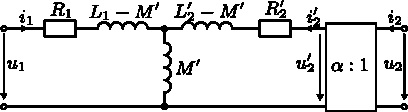
\includegraphics[width=0.99\textwidth]{fig/lec04/Transformer_T_ECD_gen_transf.pdf}
				\end{column}
				\begin{column}{0.35\textwidth}
					\caption{\raggedright T-type ECD of a transformer with transformed secondary side variables for some arbitrary transformation factor $\alpha$ (note that $k$ and $\sigma$ are transformation invariant.)}
					\label{fig:Transformer_T_ECD_gen_transf}
				\end{column}
			\end{columns}
		\end{figure}
\end{frame}

%%%%%%%%%%%%%%%%%%%%%%%%%%%%%%%%%%%%%%%%%%%%%%%%%%%%%%%%%%%%%
%% Transformation of the secondary side variables by the turn ratio %%
%%%%%%%%%%%%%%%%%%%%%%%%%%%%%%%%%%%%%%%%%%%%%%%%%%%%%%%%%%%%%
\begin{frame}
	\frametitle{Transformation of the secondary side variables by the turn ratio}
	With $$\alpha = \ddot{u} = N_1/N_2$$ being the turn ratio as the transformation factor, \pause we receive:
	\begin{equation}
		M' = (N_1/N_2)M = L_{1,\mathrm{m}}, \qquad L'_2 = (N_1^2/N_2^2) L_2
	\end{equation}
		with $L_{1,\mathrm{m}}$ being the primary magnetizing inductance, cf. \eqref{eq:inductance_split}. \pause Moreover, we have
	\begin{equation}
		L_1 - M' = L_{1,\sigma}, \qquad L_2' - M'2 =  (N_1^2/N_2^2) L_{2,\sigma} = L'_{2,
		\sigma}
	\end{equation}
	with $L_{1,\sigma}$ and $L_{2,\sigma}$ being the leakage inductances of the primary and secondary winding. \pause
	\begin{figure}
		\begin{columns}
			\begin{column}{0.64\textwidth}
					\centering
					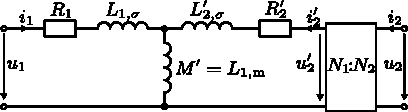
\includegraphics[width=0.99\textwidth]{fig/lec04/Transformer_T_ECD_turn_transf.pdf}
			\end{column}
			\begin{column}{0.35\textwidth}
				\caption{\raggedright T-type ECD of a transformer with $\alpha =N_1/N_2$ (note that all inductances within this model representation have a direct physical interpretation.)}
				\label{fig:Transformer_T_ECD_turn_transf}
			\end{column}
		\end{columns}
	\end{figure}	
\end{frame}

%%%%%%%%%%%%%%%%%%%%%%%%%%%%%%%%%%%%%%%%%%%%%%%%%%%%%%%%%%%%%
%% Transformation towards a single stray inductance %%
%%%%%%%%%%%%%%%%%%%%%%%%%%%%%%%%%%%%%%%%%%%%%%%%%%%%%%%%%%%%%
\begin{frame}
	\frametitle{Transformation towards a single stray inductance}
	With $$\alpha = M/L_2$$ as the transformation factor, \pause we receive:
	\begin{equation}
		L'_2 - M' = \alpha^2 L_2 - \alpha M = L_{2,\sigma} = 0,
	\end{equation}
		that is, the secondary transformed leakage inductance is vanishing. \pause Moreover, we have
	\begin{equation}
		L_1 - M' = L'_{1,\sigma}=\sigma L_1 , \qquad M'  = M^2 / L_2.
	\end{equation} 
	\onslide<5->
	With the alternative choice $\alpha = L_1/M$, the leakage inductance gets concentrated on the secondary side (not explicitly shown).
	\begin{figure}
		\onslide<4->
		\begin{columns}
			\begin{column}{0.64\textwidth}
					\centering
					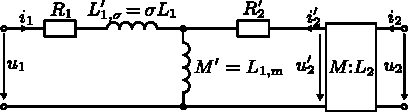
\includegraphics[width=0.99\textwidth]{fig/lec04/Transformer_T_ECD_stray_transf.pdf}
			\end{column}
			\begin{column}{0.35\textwidth}
				\caption{\raggedright T-type ECD of a transformer with $\alpha =M/L_2$}
				\label{fig:Transformer_T_ECD_stray_transf}
			\end{column}
		\end{columns}
	\end{figure}	
\end{frame}

%%%%%%%%%%%%%%%%%%%%%%%%%%%%%%%%%%%%%%%%%%%%%%%%%%%%%%%%%%%%%
%% Typical transformer core types %%
%%%%%%%%%%%%%%%%%%%%%%%%%%%%%%%%%%%%%%%%%%%%%%%%%%%%%%%%%%%%%
\begin{frame}
	\frametitle{Typical transformer core types}
	\begin{itemize}
		\item The core of a transformer typical build from laminated steel sheets (cf. \figref{fig:Eddy_currents_lamination}). Alternatively, sintered ferrite material is also used for high-frequency applications.
		\item<2-> To improve the coupling between primary and secondary winding, it is beneficial to place the windings around the same leg. Hence, the middle example in \figref{fig:Transformer_cores} will exhibit a larger leakage.
	\end{itemize}
	\begin{figure}
		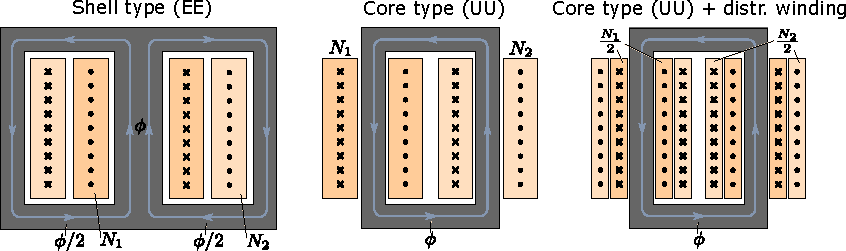
\includegraphics[width=0.9\textwidth]{fig/lec04/Transformer_cores.pdf}
		\caption{Examples of typical transformer core types}
		\label{fig:Transformer_cores}
	\end{figure}
\end{frame}

%%%%%%%%%%%%%%%%%%%%%%%%%%%%%%%%%%%%%%%%%%%%%%%%%%%%%%%%%%%%%
%% Toroidal core %%
%%%%%%%%%%%%%%%%%%%%%%%%%%%%%%%%%%%%%%%%%%%%%%%%%%%%%%%%%%%%%
\begin{frame}
	\frametitle{Toroidal core}
	\begin{figure}
		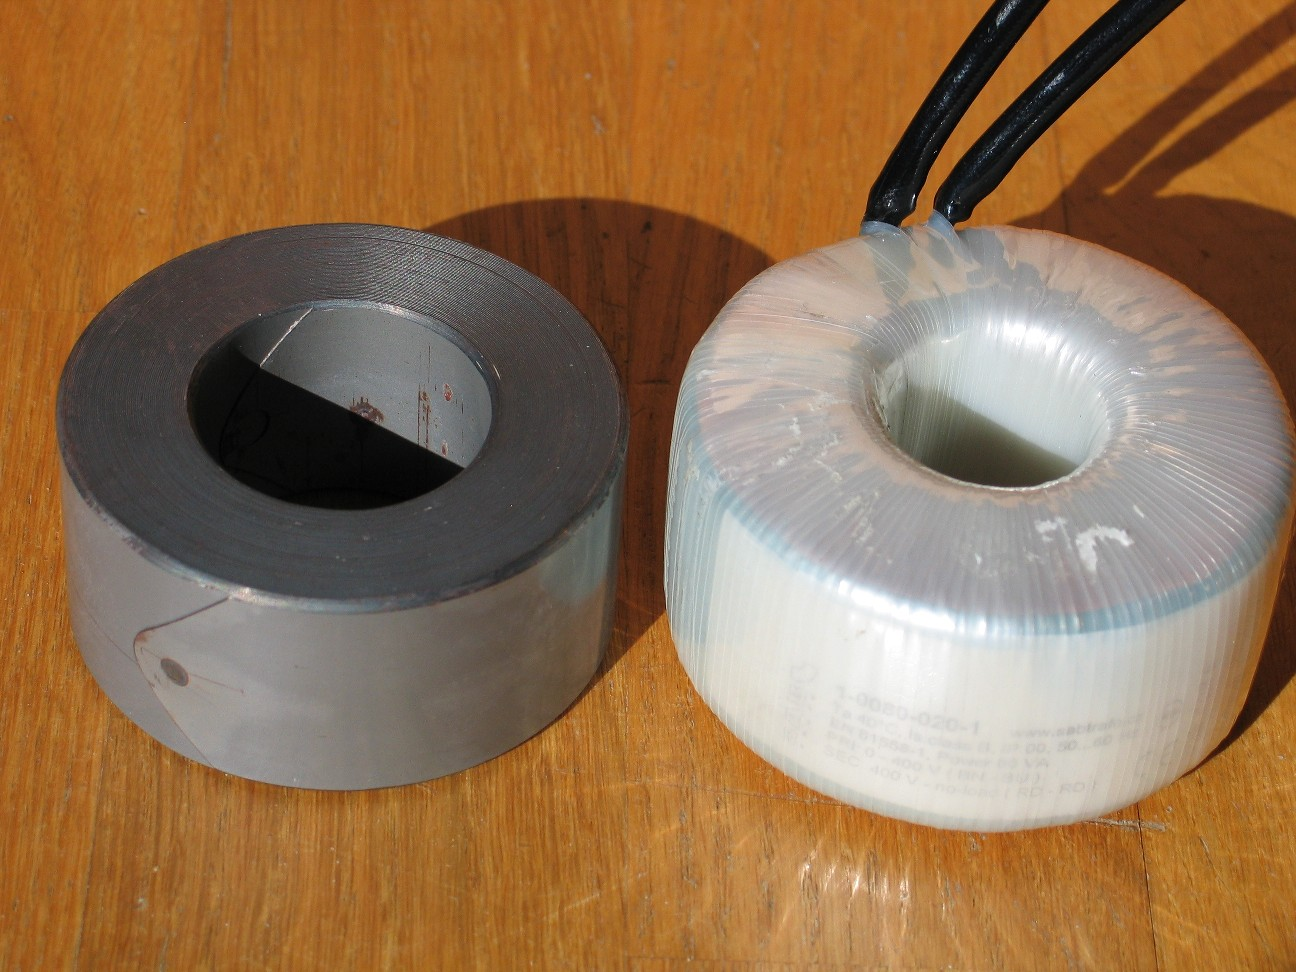
\includegraphics[height=0.7\textheight]{fig/lec04/Laminated_core_and_toroidal_transformer.jpg}
		\caption{Examples of a toroidal core and a  transformer made from it -- note the laminated, wound up steel sheets to form the toroid (source: \href{https://commons.wikimedia.org/wiki/File:Kern_und_Ringkerntrafo_100VA.JPG}{Wikimedia Commons}, public domain)}
		\label{fig:Laminated_core_and_toroidal_transformer}
	\end{figure}
\end{frame}

%%%%%%%%%%%%%%%%%%%%%%%%%%%%%%%%%%%%%%%%%%%%%%%%%%%%%%%%%%%%%
%% Typical transformer winding schemes %%
%%%%%%%%%%%%%%%%%%%%%%%%%%%%%%%%%%%%%%%%%%%%%%%%%%%%%%%%%%%%%
\begin{frame}
	\frametitle{Typical transformer winding schemes}
	\begin{itemize}
		\item The below examples show improving magnetic coupling (lower leakage) from left to right due to the reducing effective distance between the turns of the primary and secondary winding.
		\item<2-> Beyond these examples, various winding variations (e.g., a combination of the below schemes) are used to optimize the transformer design for specific applications. 
	\end{itemize}
	\vspace{0.5em}
	\begin{figure}
		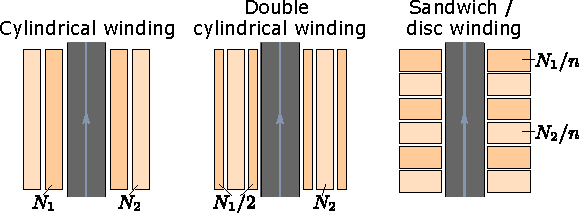
\includegraphics[width=0.7\textwidth]{fig/lec04/Transformer_winding_types.pdf}
		\caption{Examples of typical transformer winding schemes}
		\label{fig:Transformer_winding_types}
	\end{figure}
\end{frame}


%%%%%%%%%%%%%%%%%%%%%%%%%%%%%%%%%%%%%%%%%%%%%%%%%%%%%%%%%%%%%
%% Core loss model (hyteresis and eddy current losses) %%
%%%%%%%%%%%%%%%%%%%%%%%%%%%%%%%%%%%%%%%%%%%%%%%%%%%%%%%%%%%%%
\begin{frame}
	\frametitle{Core loss model (hysteresis and eddy current losses)}
	To also consider the iron losses inside the transformer core, a first-order model with the additional core loss resistance $R_{\mathrm{c}}$ can be introduced:
	\begin{equation}
		P_{\mathrm{l,c}} \approx R_{\mathrm{c}} I_{\mathrm{c}}^2 \approx \frac{U_1^2}{R_{\mathrm{c}}}. 
	\end{equation}
	Here, we consider a pure sinusoidal operation with $I_\mathrm{c}$ and $U_1$ being root-mean-square (RMS) values. \pause Obviously, this is only a very rough model approximation (compare \figref{fig:Hyteresis_curve_full} and \figref{fig:Eddy_currents_lamination}), but for many transformer designs the core losses can be significant and neglecting them completely would not be justified. 
	\begin{figure}
		\onslide<1->
		\begin{columns}
			\begin{column}{0.64\textwidth}
					\centering
					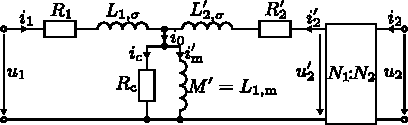
\includegraphics[width=0.99\textwidth]{fig/lec04/Transformer_T_ECD_core_losses.pdf}
			\end{column}
			\begin{column}{0.35\textwidth}
				\caption{\raggedright T-type ECD of a transformer with an additional core loss resistance $R_{\mathrm{c}}$}
				\label{fig:Transformer_T_ECD_core_losses}
			\end{column}
		\end{columns}
	\end{figure}	
\end{frame}

%%%%%%%%%%%%%%%%%%%%%%%%%%%%%%%%%%%%%%%%%%%%%%%%%%%%%%%%%%%%%
%% Transformer model parameterization via measurements -- open circuit test %%
%%%%%%%%%%%%%%%%%%%%%%%%%%%%%%%%%%%%%%%%%%%%%%%%%%%%%%%%%%%%%
\begin{frame}
	\frametitle{Transformer model parameterization via measurements -- open-circuit test}
	\pause
	Applying a sinusoidal test voltage $U_{1,\mathrm{o}}$ and several measurement devices during an open-circuit arrangement, we can determine
	\begin{equation}
		\ddot{u} \approx \frac{U_{1,\mathrm{o}}}{U_{2,\mathrm{o}}} = \frac{N_1}{N_2}, \quad S_{1,\mathrm{o}} = U_{1,\mathrm{o}} I_{1,\mathrm{o}}, \quad \cos(\varphi_{\mathrm{o}}) = \frac{P_{1,\mathrm{o}}}{U_{1,\mathrm{o}} I_{1,\mathrm{o}}}
	\end{equation} 
	with $P_{1,\mathrm{o}}$ being the active input power consumed by the transformer and $\cos(\varphi_{\mathrm{o}})$ is the power factor. \pause With the assumptions $R_1 << R_\mathrm{c}$ and $L_{1,\sigma} << M'$, we can approximate 
	\begin{equation}
		R_{\mathrm{c}} \approx \frac{U_{1,\mathrm{o}}^2}{P_{1,\mathrm{o}}}, \quad X_{M'} = \omega_{\mathrm{el}} M'  \approx \frac{U_{1,\mathrm{o}}}{I_{1,\mathrm{o}} \sin(\varphi_{\mathrm{o}})}
	\end{equation}
	given the angular frequency $\omega_{\mathrm{el}} = 2\pi f_{\mathrm{el}}$ and the reactance $X_{M'}$ of the mutual inductance.
	\begin{figure}
		\onslide<1->
		\begin{columns}
			\begin{column}{0.64\textwidth}
					\centering
					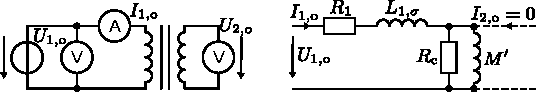
\includegraphics[width=0.99\textwidth]{fig/lec04/Transformer_open_circuit_test.pdf}
			\end{column}
			\begin{column}{0.35\textwidth}
				\caption{\raggedright Open-circuit (no-load) test: measuring circuit and its ECD}
				\label{fig:Transformer_open_circuit_test}
			\end{column}
		\end{columns}
	\end{figure}	
\end{frame}

%%%%%%%%%%%%%%%%%%%%%%%%%%%%%%%%%%%%%%%%%%%%%%%%%%%%%%%%%%%%%
%% Transformer model parameterization via measurements -- short circuit test %%
%%%%%%%%%%%%%%%%%%%%%%%%%%%%%%%%%%%%%%%%%%%%%%%%%%%%%%%%%%%%%
\begin{frame}
	\frametitle{Transformer model parameterization via measurements -- short-circuit test}
	\pause
	Short-circuiting the secondary and applying a sinusoidal test voltage $U_{1,\mathrm{s}}$,  we can determine
	\begin{equation}
		Z_\mathrm{s} = \sqrt{(R_1+R'_2)^2 + (X_{L_{1,\sigma}} + X_{L'_{2,\sigma}})^2}, \quad  \cos(\varphi_{\mathrm{s}}) = \frac{P_{1,\mathrm{s}}}{U_{1,\mathrm{s}} I_{1,\mathrm{s}}}
	\end{equation} 
	with $Z_\mathrm{s}$ being the short-circuit impedance while assuming that the impedance across $M'$ and $R_{\mathrm{c}}$ is much larger, i.e., the short-circuit current will not flow via this branch. \pause Hence, we have
	\begin{equation}
		R_1+R'_2 = Z_\mathrm{s}\cos(\varphi_{\mathrm{s}}), \quad X_{L_{1,\sigma}} + X_{L'_{2,\sigma}} = Z_\mathrm{s} \sin(\varphi_{\mathrm{s}}).
	\end{equation}  
	\pause
	Since we have four remaining unknown component values but only two independent equations, we additionally assume a symmetrical transformer design, leading to
	\begin{equation}
		R_1 = R'_2 = \frac{1}{2}Z_\mathrm{s}\cos(\varphi_{\mathrm{s}}), \quad \omega_{\mathrm{el}}L_{1,\sigma} =  X_{L_{1,\sigma}} = \omega_{\mathrm{el}}L'_{2,\sigma} = X_{L'_{2,\sigma}} = \frac{1}{2} Z_\mathrm{s} \sin(\varphi_{\mathrm{s}}).
	\end{equation}
	\vspace{-0.3cm}
	\begin{figure}
		\onslide<1->
		\begin{columns}
			\begin{column}{0.64\textwidth}
					\centering
					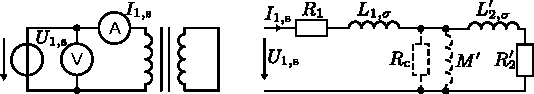
\includegraphics[width=0.99\textwidth]{fig/lec04/Transformer_short_circuit_test.pdf}
			\end{column}
			\begin{column}{0.35\textwidth}
				\caption{\raggedright Short-circuit test: measuring circuit and its ECD}
				\label{fig:Transformer_short_circuit_test}
			\end{column}
		\end{columns}
	\end{figure}	
\end{frame}

%%%%%%%%%%%%%%%%%%%%%%%%%%%%%%%%%%%%%%%%%%%%%%%%%%%%%%%%%%%%%
%% Further short-circuit considerations %%
%%%%%%%%%%%%%%%%%%%%%%%%%%%%%%%%%%%%%%%%%%%%%%%%%%%%%%%%%%%%%
\begin{frame}
	\frametitle{Further short-circuit considerations}
	Typically the short-circuit test voltage $U_{1,\mathrm{s}}$ is limited such that the short-circuit current $I_{1,\mathrm{s}}$ is reaching its nominal value $I_{1,\mathrm{n}}$:
	\begin{equation}
		U_{1,\mathrm{s}} = u_{1,\mathrm{s}} U_{1,\mathrm{n}}, \quad I_{1,\mathrm{s}} = \frac{U_{1,\mathrm{s}}}{Z_\mathrm{s}} = I_{1,\mathrm{n}}.
	\end{equation}
	Here, $u_{1,\mathrm{s}}$ is the relative short-circuit voltage w.r.t. the nominal voltage $U_{1,\mathrm{n}}$. \pause Typical values are $u_{1,\mathrm{s}} = 3 \ldots 13 \, \%.$ \pause
	\\[1em]
	While the short-circuit test is conducted with a reduced primary voltage, the prospective short-circuit (PSC) current during normal operation (typical as a fault result) can be significantly higher:
	\begin{equation}
		I_{1,\mathrm{psc}} = \frac{U_{1,\mathrm{n}}}{Z_\mathrm{s}} = \frac{U_{1,\mathrm{s}}}{Z_\mathrm{s}} = \frac{I_{1,\mathrm{n}}}{u_{1,\mathrm{s}}}.
	\end{equation}  \pause
	Hence, the transformer parameters $Z_\mathrm{s}$ and $u_{1,\mathrm{s}}$ are crucial for the short-circuit behavior and the protection coordination of the transformer. Lower bounds are typically enforced by standards to prevent catastrophic damages, in particular in the electrical energy sector.
\end{frame}


%%%%%%%%%%%%%%%%%%%%%%%%%%%%%%%%%%%%%%%%%%%%%%%%%%%%%%%%%%%%%
%% Voltage transformer application: measuring high AC voltages %%
%%%%%%%%%%%%%%%%%%%%%%%%%%%%%%%%%%%%%%%%%%%%%%%%%%%%%%%%%%%%%
\begin{frame}
	\frametitle{Voltage transformer application: measuring high AC voltages}
	If the voltage to be measured is too high for direct measurement, a voltage transformer can be used to step down the voltage to a suitable level:
	$$u_2(t) = \frac{1}{\ddot{u}} u_1(t).$$
	\pause
	Hence, we choose $\ddot{u} > 1$. \pause Moreover, the voltage sensor on the secondary side comes with a high internal resistance $R_\mathrm{i}$ to avoid a significant current and, therefore, power flow. Neglecting the leakage inductance, we can model the voltage transformer as shown in \figref{fig:Voltage_transformer_meas_ECD} with
	$$	R'_\mathrm{i} = \ddot{u}^2R_\mathrm{i}, \qquad R'_2 = \ddot{u}^2R_2, \qquad M' = L_{1,\mathrm{m}}.$$
	\pause
	The primary RL circuit represents a high-pass filter for the voltage signal, i.e., the transformer is only suitable for AC signals with $\omega_{\mathrm{el}} > R_1/M'$ (cutoff frequency).
	\begin{figure}
		\onslide<1->
		\begin{columns}
			\begin{column}{0.64\textwidth}
					\centering
					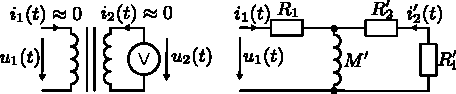
\includegraphics[width=0.95\textwidth]{fig/lec04/Voltage_transformer_meas_ECD.pdf}
			\end{column}
			\begin{column}{0.35\textwidth}
				\caption{\raggedright Voltage transformer measuring circuit and its ECD (represented as transformed quantities with $\alpha = N_1/N_2$)}
				\label{fig:Voltage_transformer_meas_ECD}
			\end{column}
		\end{columns}
	\end{figure}
\end{frame}

%%%%%%%%%%%%%%%%%%%%%%%%%%%%%%%%%%%%%%%%%%%%%%%%%%%%%%%%%%%%%
%% Current transformer application: measuring high AC currents %%
%%%%%%%%%%%%%%%%%%%%%%%%%%%%%%%%%%%%%%%%%%%%%%%%%%%%%%%%%%%%%
\begin{frame}
	\frametitle{Current transformer application: measuring high AC currents}
	If the current to be measured is too high for direct measurement, a current transformer can be used to step down the current to a suitable level:
	$$i_2(t) = \ddot{u} i_1(t).$$ \pause
	Hence, we choose $\ddot{u} < 1$. \pause Moreover, the current sensor on the secondary side comes with a minimal internal resistance $R_\mathrm{i}$ to avoid a significant ohmic power losses. Likewise, the transformer should be designed for low $R_1$ and $R_2$ (e.g., $N_1=1$ on the primary and sufficiently large cable cross-sections).\\ \pause
	\vspace{1em}
	The secondary RL circuit represents a high-pass filter for the current signal, i.e., the transformer is only suitable for AC signals with $\omega_{\mathrm{el}} > (R'_2 + R'_\mathrm{i})/M'$ (cutoff frequency).
	\begin{figure}
		\onslide<1->
		\begin{columns}
			\begin{column}{0.64\textwidth}
					\centering
					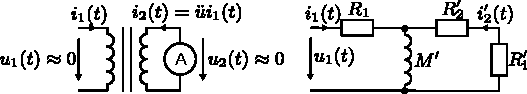
\includegraphics[width=0.99\textwidth]{fig/lec04/Current_transformer_meas_ECD.pdf}
			\end{column}
			\begin{column}{0.35\textwidth}
				\caption{\raggedright Current transformer measuring circuit and its ECD (represented as transformed quantities with $\alpha = N_1/N_2$)}
				\label{fig:Current_transformer_meas_ECD}
			\end{column}
		\end{columns}
	\end{figure}
\end{frame}

%%%%%%%%%%%%%%%%%%%%%%%%%%%%%%%%%%%%%%%%%%%%%%%%%%%%%%%%%%%%%
%% Connection nomenclature and tapped transformer %%
%%%%%%%%%%%%%%%%%%%%%%%%%%%%%%%%%%%%%%%%%%%%%%%%%%%%%%%%%%%%%
\begin{frame}
	\frametitle{Connection nomenclature and tapped transformer}
	\begin{columns}[b]
		\begin{column}{0.45\textwidth}
			\begin{figure}
				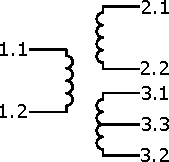
\includegraphics[width=0.45\textwidth]{fig/lec04/Connection_nomenclature_single_phase_transformer.pdf}
				\vspace{1cm}
				\caption{Connection nomenclature of single-phase transformers (the lower secondary side connection represents a tapped winding)}
				\label{fig:Connection_nomenclature_single_phase_transformer}
			\end{figure}
		\end{column}
        \hfill \pause
		\begin{column}{0.55\textwidth}
			\begin{figure}
				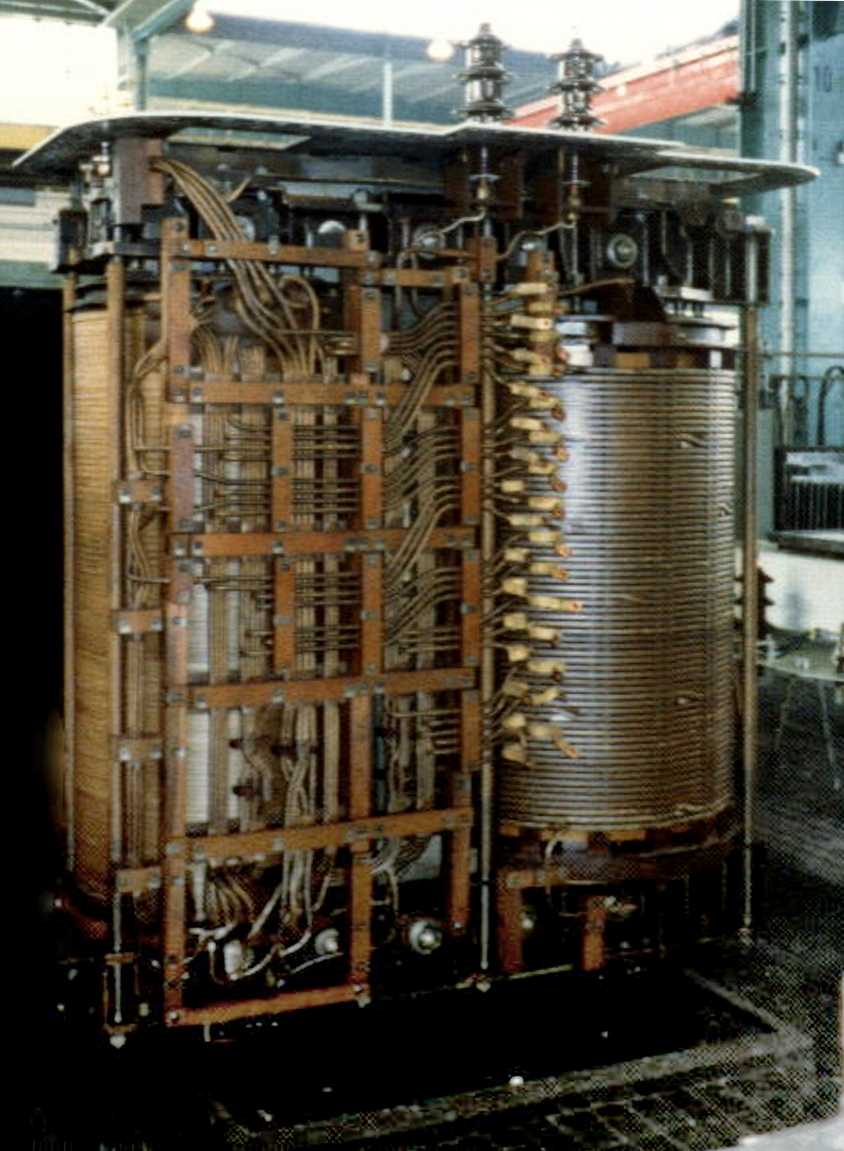
\includegraphics[height=0.6\textheight]{fig/lec04/Taped_transformer_train_example.jpg}
				\caption{Tapped transformer with multiple taps on the secondary side for a train drive application (source: \href{https://de.wikipedia.org/wiki/Datei:TrafoAW-2.jpg}{Wikimedia Commons}, Saibo, \href{https://creativecommons.org/licenses/by-sa/3.0/deed.en}{CC BY-SA 3.0})}
				\label{fig:Taped_transformer_train_example}
			\end{figure}
		\end{column}
	\end{columns}
\end{frame}

%%%%%%%%%%%%%%%%%%%%%%%%%%%%%%%%%%%%%%%%%%%%%%%%%%%%%%%%%%%%%
%% Autotransformer %%
%%%%%%%%%%%%%%%%%%%%%%%%%%%%%%%%%%%%%%%%%%%%%%%%%%%%%%%%%%%%%
\begin{frame}
	\frametitle{Autotransformer}
	\begin{columns}
		\begin{column}{0.575\textwidth}
            \begin{itemize}
                \item Uses a common winding for both primary and secondary side with one or multiple taps.
                \item No galvanic isolation between primary and secondary side.
                \item The autotransformer can be used to step-up or step-down the voltage.
            \end{itemize}
			\begin{figure}
                \centering
                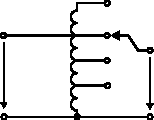
\includegraphics[height=0.3\textheight]{fig/lec04/Autotransformer_symbol.pdf}
                \caption{Simplified autotransformer representation}
            \end{figure}
		\end{column}
        \hfill
		\begin{column}{0.425\textwidth}
            \vspace{-0.2cm}
			\onslide<2->\begin{figure}
				\centering
				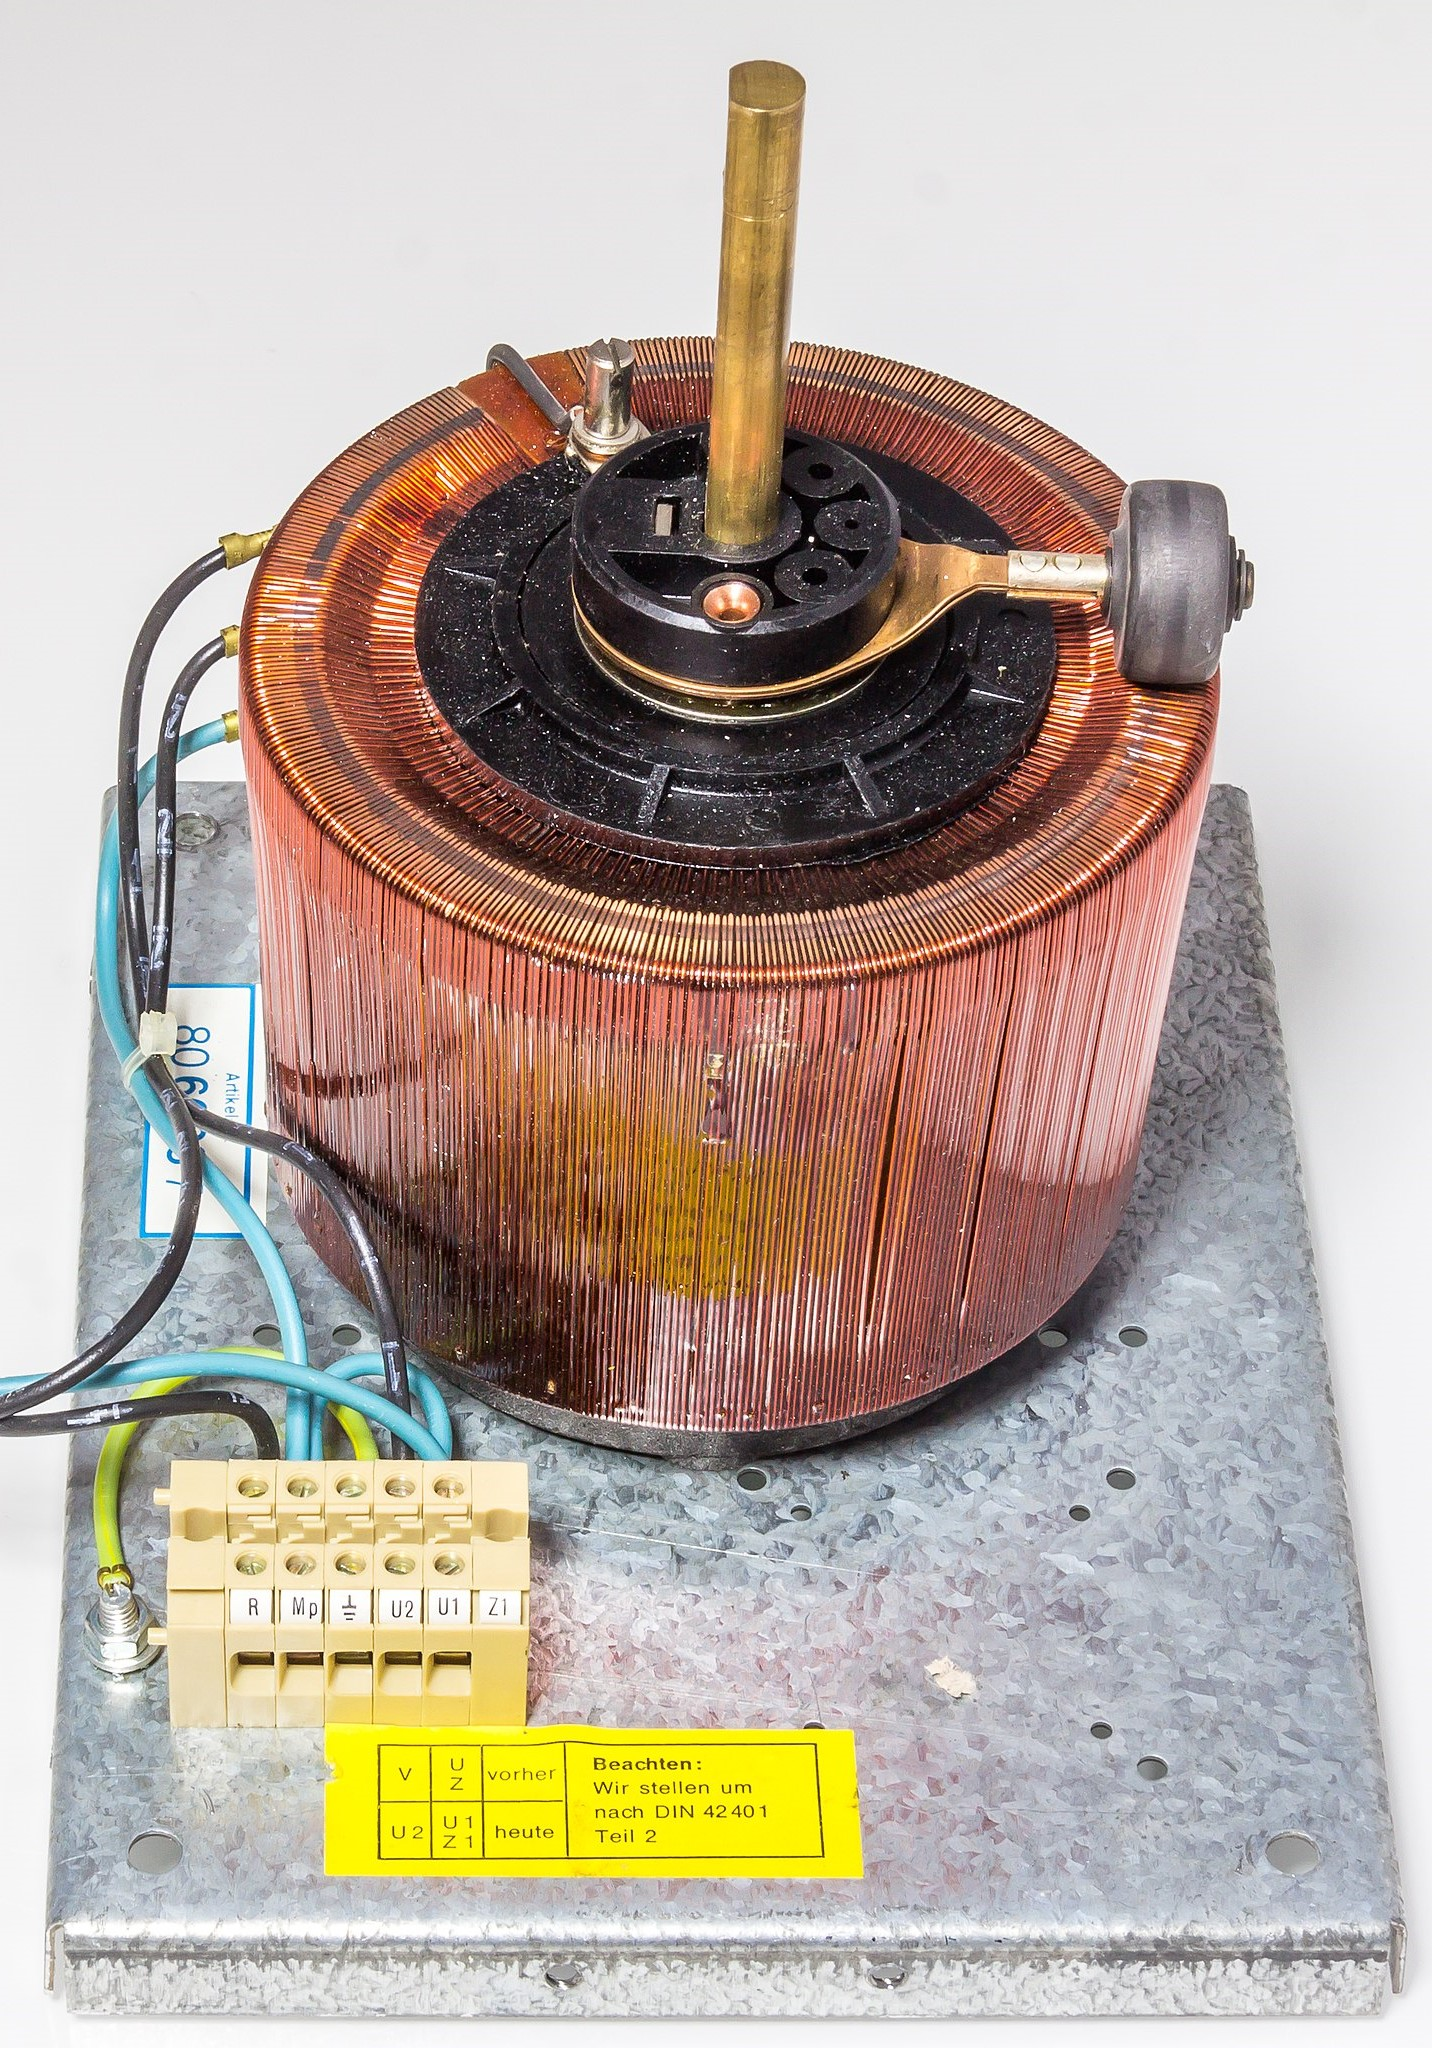
\includegraphics[height=0.6\textheight]{fig/lec04/Variable_autotransformer.jpg}
				\caption{Exemplary autotransformer (source: \href{https://de.wikipedia.org/wiki/Datei:Variable_autotransformer_0-220_V,_4_A,_880_VA-1095.jpg}{Wikimedia Commons}, R.~Spekking, \href{https://creativecommons.org/licenses/by-sa/4.0/deed.en}{CC BY-SA 4.0})}
			\end{figure}
		\end{column}
		\end{columns}
\end{frame}

%%%%%%%%%%%%%%%%%%%%%%%%%%%%%%%%%%%%%%%%%%%%%%%%%%%%%%%%%%%%%
%% Autotransformer -- step-down configuration %%
%%%%%%%%%%%%%%%%%%%%%%%%%%%%%%%%%%%%%%%%%%%%%%%%%%%%%%%%%%%%%
\begin{frame}
	\frametitle{Autotransformer -- step-down configuration}
	Assuming idealized conditions (no leakage, no losses), the apparent power of the standard transformer $S$ and of the autotransformer $S_\mathrm{at}$ are:
	\begin{equation}
		S= U_1 I_1 = U_2 I_2, \qquad S_\mathrm{at} = (U_1+U_2) I_1 = U_2 (I_2-I_1).
		\label{eq:apparent_power_autotransformer}
	\end{equation}
	\begin{figure}
		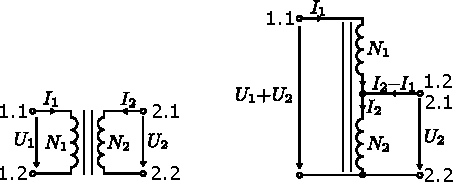
\includegraphics[width=0.6\textwidth]{fig/lec04/Autotransformer_step_down.pdf}
		\caption{Step-down autotransformer made from a standard two-winding transformer by connecting 1.2 from the primary to 2.1 on the secondary side}
		\label{fig:Autotransformer_step_down}
	\end{figure}
\end{frame}

%%%%%%%%%%%%%%%%%%%%%%%%%%%%%%%%%%%%%%%%%%%%%%%%%%%%%%%%%%%%%
%% Autotransformer -- step-down configuration  (cont.) %%
%%%%%%%%%%%%%%%%%%%%%%%%%%%%%%%%%%%%%%%%%%%%%%%%%%%%%%%%%%%%%
\begin{frame}
	\frametitle{Autotransformer -- step-down configuration  (cont.)}
	From \eqref{eq:apparent_power_autotransformer} we can express the autotransformer apparent power $S_\mathrm{at}$ in terms of the standard transformer apparent power $S$:
	\begin{equation}
		S_\mathrm{at} = (U_1+U_2) I_1 = S + U_2 I_1 = S + U_1 I_1 \frac{U_2}{U_1} = S(1+\frac{1}{\ddot{u}}).
	\end{equation}
	Here, $\ddot{u}$ is the (idealized) voltage transformation ratio of the standard transformer -- compare \eqref{eq:voltage_transformation_ratio}. \pause Hence, we can express the apparent power of the autotransformer in terms of the standard transformer apparent power:
	\begin{equation}
		\frac{S_\mathrm{at}}{S} = 1+\frac{1}{\ddot{u}} = 1 + \frac{N_2}{N_1}.
	\end{equation} \pause
	Since $N_2 / N_1 > 0$ the autotransformer can transfer more apparent power than the standard transformer since the autotransformer combines two power transfer mechanisms: \pause
	\begin{itemize}
		\item the apparent power $U_1 I_1$ is transferred via the magnetic coupling (induction) and \pause
		\item the apparent power $U_2 I_1$ is transferred via the electrical conduction between primary and secondary (not available in the galvanically-isolated standard transformer).
	\end{itemize}
\end{frame}

%%%%%%%%%%%%%%%%%%%%%%%%%%%%%%%%%%%%%%%%%%%%%%%%%%%%%%%%%%%%%
%% Autotransformer -- step-up configuration %%
%%%%%%%%%%%%%%%%%%%%%%%%%%%%%%%%%%%%%%%%%%%%%%%%%%%%%%%%%%%%%
\begin{frame}
	\frametitle{Autotransformer -- step-up configuration}
	The apparent power of the step-up autotransformer is 
	\begin{equation}
		S_\mathrm{at} = U_1 (I_1-I_2) = (U_1+U_2)I_2 = S(1+\frac{U_1}{U_2})= S(1+\ddot{u})= S(1+\frac{N_1}{N_2}).
	\end{equation}
	Likewise to the step-down autotransformer, the step-up autotransformer can transfer more apparent power than the standard transformer.
	\begin{figure}
		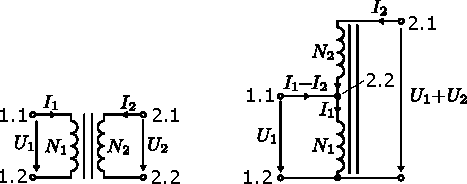
\includegraphics[width=0.6\textwidth]{fig/lec04/Autotransformer_step_up.pdf}
		\caption{Step-up autotransformer made from a standard two-winding transformer by connecting 1.1 from the primary to 2.2 on the secondary side}
		\label{fig:Autotransformer_step_up}
	\end{figure}
\end{frame}

%%%%%%%%%%%%%%%%%%%%%%%%%%%%%%%%%%%%%%%%%%%%%%%%%%%%%%%%%%%%%
%% Autotransformer remarks%%
%%%%%%%%%%%%%%%%%%%%%%%%%%%%%%%%%%%%%%%%%%%%%%%%%%%%%%%%%%%%%
\begin{frame}
	\frametitle{Autotransformer remarks}
	\begin{columns}
		\begin{column}{0.5\textwidth}
			The previous analysis has revealed that the apparent power boost over the standard transformer is significant if
            \begin{itemize}
                \item $N_2 >> N_1$ (step-down case) or
                \item $N_1 >> N_2$ (step-up case),
            \end{itemize}
		that is, the autotransformer's input and output voltage have only a small difference. \pause In this case, the autotransformer can be more efficient and cost-effective than the standard transformer (at the drawback of the lacking galvanic isolation).
		\end{column}
        \hfill
		\begin{column}{0.5\textwidth}
			\onslide<1->
			\begin{figure}
				\centering
				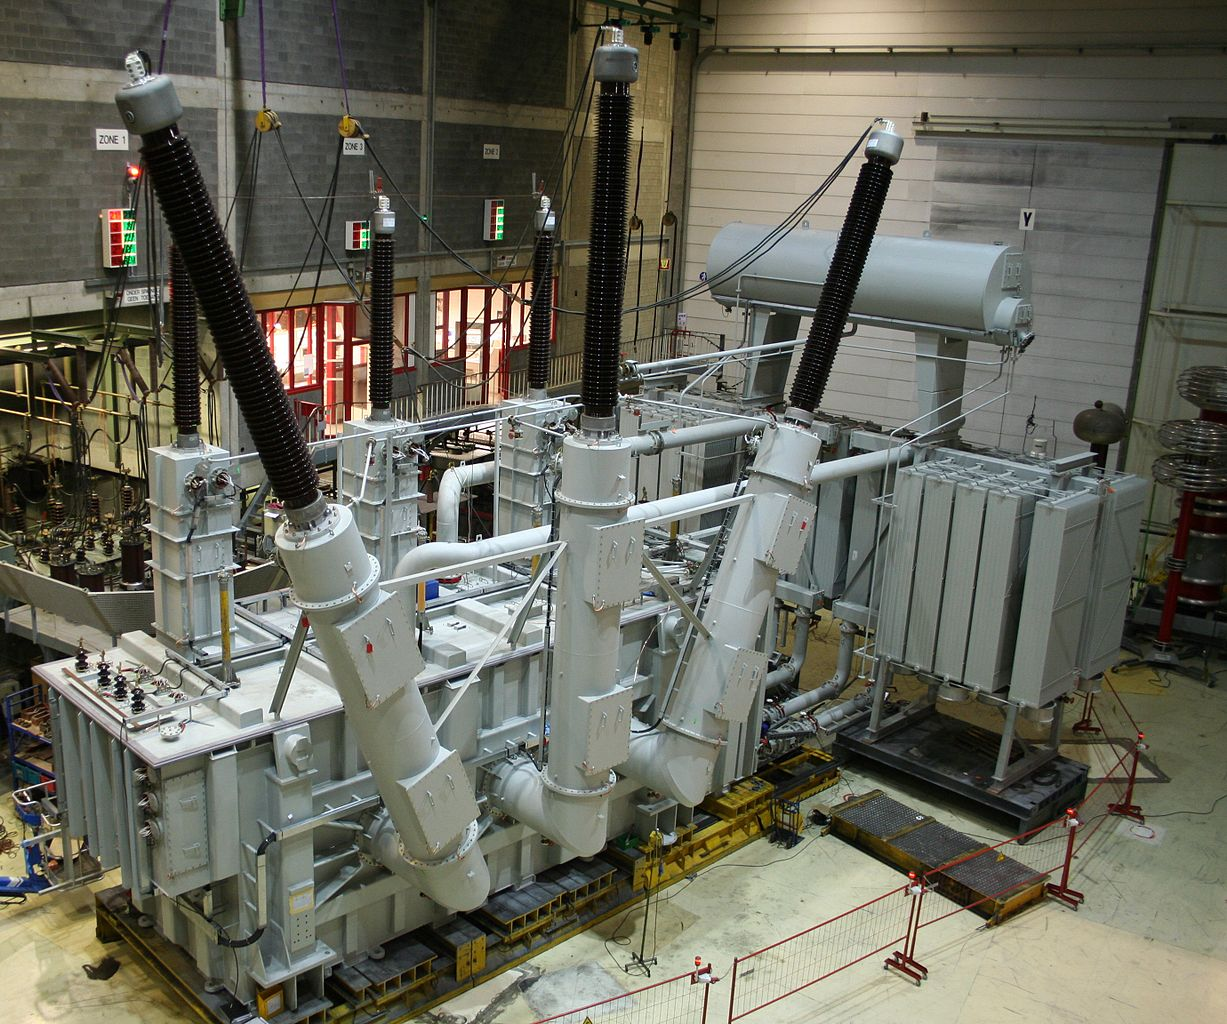
\includegraphics[width=0.85\textwidth]{fig/lec04/Autotransformer_three_phase.jpg}
				\caption{\SI{750}{\mega\volt\ampere}, \SI{380}{\kilo\volt} / \SI{230}{\kilo\volt} three-phase autotransformer (source: \href{https://commons.wikimedia.org/wiki/File:CG_Autotrafo_4002904.jpg}{Wikimedia Commons}, P.~Mertens, \href{https://creativecommons.org/licenses/by-sa/3.0/deed.en}{CC BY-SA 3.0})}
			\end{figure}
		\end{column}
	\end{columns}
\end{frame}

%%%%%%%%%%%%%%%%%%%%%%%%%%%%%%%%%%%%%%%%%%%%%%%%%%%%%%%%%%%%%
%% Autotransformer remarks (cont.)%%
%%%%%%%%%%%%%%%%%%%%%%%%%%%%%%%%%%%%%%%%%%%%%%%%%%%%%%%%%%%%%
\begin{frame}
	\frametitle{Autotransformer remarks (cont.)}
	Another challenge of the autotransformer is its short-circuit behavior. From the step-up case we know:
	$$ S_\mathrm{at} = S(1+\frac{N_1}{N_2}).$$ 
	\pause
	Dividing both sides by $U_1$ delivers
	\begin{equation}
		I_{1,\mathrm{at}} = I_{1}(1+\frac{N_1}{N_2})
	\end{equation}
	\pause
	Hence, in case of a short circuit the steady-state current of the autotransformer is $1+N_1/N_2$ times higher than the standard transformer:
	\begin{equation}
		I_{1,\mathrm{at,psc}} = I_{1,\mathrm{psc}}(1+\frac{N_1}{N_2}).
	\end{equation}
	\pause
	The same applies to the step-down case. Therefore, the autotransformer may require additional short-circuit protection measures to prevent damages (e.g., additional choke).
\end{frame}

%%%%%%%%%%%%%%%%%%%%%%%%%%%%%%%%%%%%%%%%%%%%%%%%%%%%%%%%%%%%%
%% Three-phase transformer %%
%%%%%%%%%%%%%%%%%%%%%%%%%%%%%%%%%%%%%%%%%%%%%%%%%%%%%%%%%%%%%
\begin{frame}
	\frametitle{Three-phase transformer}
	\begin{figure}
		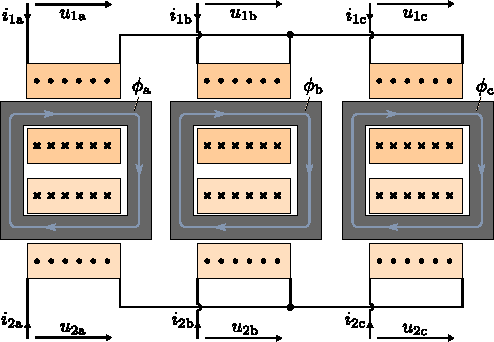
\includegraphics[width=0.6\textwidth]{fig/lec04/Three_phase_transformer_simple.pdf}
		\caption{Simple three-phase transformer with three independent single-phase transformers connected in star both on the primary and secondary side}
		\label{fig:Three_phase_transformer_simple}
	\end{figure}
\end{frame}

%%%%%%%%%%%%%%%%%%%%%%%%%%%%%%%%%%%%%%%%%%%%%%%%%%%%%%%%%%%%%
%% Three-phase transformer with five legs %%
%%%%%%%%%%%%%%%%%%%%%%%%%%%%%%%%%%%%%%%%%%%%%%%%%%%%%%%%%%%%%
\begin{frame}
	\frametitle{Three-phase transformer with five legs}
	\begin{figure}
		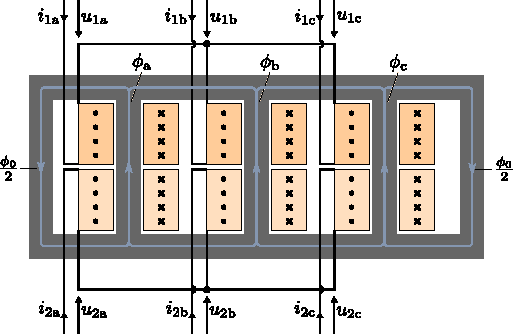
\includegraphics[height=0.75\textheight]{fig/lec04/Three_phase_transformer_5_legs.pdf}
		\caption{Three-phase five-leg transformer connected in star both on the primary and secondary side}
		\label{fig:Three_phase_transformer_5_legs}
	\end{figure}
\end{frame}


%%%%%%%%%%%%%%%%%%%%%%%%%%%%%%%%%%%%%%%%%%%%%%%%%%%%%%%%%%%%%
%% Three-phase transformer with five legs (cont.) %%
%%%%%%%%%%%%%%%%%%%%%%%%%%%%%%%%%%%%%%%%%%%%%%%%%%%%%%%%%%%%%
\begin{frame}
	\frametitle{Three-phase transformer with five legs (cont.)}
	Obviously, the three-phase five-leg design from \figref{fig:Three_phase_transformer_5_legs} can save space and material compared to the three independent single-phase transformers from \figref{fig:Three_phase_transformer_simple}. However, there might be a zero flux component
	\begin{equation}
		\phi_0(t) = \phi_\mathrm{a}(t) + \phi_\mathrm{b}(t) + \phi_\mathrm{c}(t)  
	\end{equation} 
	flowing via the winding-free legs. \pause This zero flux component can be avoided if the primary and secondary side are connected both in star configuration
	$$ i_{1\mathrm{a}}(t)+i_{1\mathrm{b}}(t)+i_{1\mathrm{c}}(t)=0, \qquad i_{2\mathrm{a}}(t)+i_{2\mathrm{b}}(t)+i_{2\mathrm{c}}(t)=0$$
	\pause
	and if the magnetic reluctances $\Lambda_\mathrm{m}$ of the three main legs are equal (i.e., symmetric design, no saturation):
	\begin{equation*}
		\phi_0 = \phi_\mathrm{a} + \phi_\mathrm{b} + \phi_\mathrm{c} = \Lambda_\mathrm{m} N_1 \left(i_{1\mathrm{a}}(t)+i_{1\mathrm{b}}(t)+i_{1\mathrm{c}}(t)\right)+\Lambda_\mathrm{m} N_2 \left(i_{2\mathrm{a}}(t)+i_{2\mathrm{b}}(t)+i_{2\mathrm{c}}(t)\right) = 0.
	\end{equation*}
\end{frame}

%%%%%%%%%%%%%%%%%%%%%%%%%%%%%%%%%%%%%%%%%%%%%%%%%%%%%%%%%%%%%
%% Three-phase transformer with three legs (double star connection) %%
%%%%%%%%%%%%%%%%%%%%%%%%%%%%%%%%%%%%%%%%%%%%%%%%%%%%%%%%%%%%%
\begin{frame}
	\frametitle{Three-phase transformer with three legs (double star connection)}
	\begin{columns}
		\begin{column}{0.4\textwidth}
           \begin{itemize}
				\item If the flux zero component $\phi_0$ can be avoided, a three-leg design as shown in \figref{fig:Three_phase_transformer_3_legs_star} can be used. \pause
				\item However, if $\phi_0 \neq 0$ due to an asymmetric design, magnetic saturation or non-ideal symmetrical operation, the zero component will act as a stray field leaving the core. \pause
				\item This can lead to increased losses in auxiliary components (e.g., housing) and electromagnetic interference issues.
			\end{itemize}
		\end{column}
        \hfill
		\begin{column}{0.6\textwidth}
			\onslide<1->
			\begin{figure}
				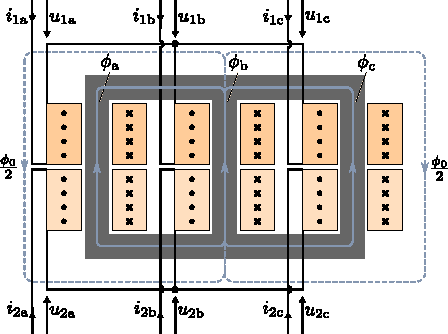
\includegraphics[height=0.7\textheight]{fig/lec04/Three_phase_transformer_3_legs_star.pdf}
				\caption{Three-phase three-leg transformer connected in star both on the primary and secondary side}
				\label{fig:Three_phase_transformer_3_legs_star}
			\end{figure}
		\end{column}
	\end{columns}
\end{frame}

%%%%%%%%%%%%%%%%%%%%%%%%%%%%%%%%%%%%%%%%%%%%%%%%%%%%%%%%%%%%%
%% Three-phase transformer with three legs (star-delta connection) %%
%%%%%%%%%%%%%%%%%%%%%%%%%%%%%%%%%%%%%%%%%%%%%%%%%%%%%%%%%%%%%
\begin{frame}
	\frametitle{Three-phase transformer with three legs (star-delta connection)}
	\begin{columns}
		\begin{column}{0.4\textwidth}
 			If the primary or secondary side is connected in delta configuration, this side can carry a zero sequence current:
			\begin{equation*}
				i_0 = \frac{1}{3}\left(i_\mathrm{a}(t) + i_\mathrm{b}(t) + i_\mathrm{c}(t)\right) \neq 0 .
			\end{equation*}
			\pause
			This zero sequence current would not be visible in the phase conductors:
			\begin{equation}
				\begin{split}
					i_\mathrm{ab} &= i_\mathrm{a} - i_\mathrm{b}, \\ i_\mathrm{bc} &= i_\mathrm{b} - i_\mathrm{c},\\ i_\mathrm{ca} &= i_\mathrm{c} - i_\mathrm{a}.
				\end{split}
				\label{eq:zero_sequence_currents_phase_transformer}
			\end{equation}
		\end{column}
        \hfill
		\begin{column}{0.6\textwidth}
			\onslide<1->
			\begin{figure}
				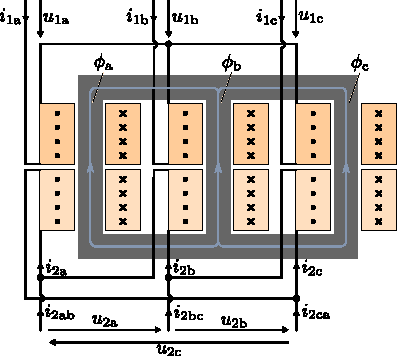
\includegraphics[height=0.7\textheight]{fig/lec04/Three_phase_transformer_3_legs_star_delta.pdf}
				\caption{Three-phase three-leg transformer connected in a star-delta configuration (delta on secondary is exemplary)}
				\label{fig:Three_phase_transformer_3_legs_star_delta}
			\end{figure}
		\end{column}
	\end{columns}
\end{frame}

%%%%%%%%%%%%%%%%%%%%%%%%%%%%%%%%%%%%%%%%%%%%%%%%%%%%%%%%%%%%%
%% Zero flux and zero current components in three-phase transformers %%
%%%%%%%%%%%%%%%%%%%%%%%%%%%%%%%%%%%%%%%%%%%%%%%%%%%%%%%%%%%%%
\begin{frame}
	\frametitle{Zero flux and zero current components in three-phase transformers}
	Based on \eqref{eq:zero_sequence_currents_phase_transformer} the winding currents on the delta side becomes
	\begin{equation}		
			i_\mathrm{a} = i_0 + \frac{1}{3}\left(i_\mathrm{ab}-i_\mathrm{ca}\right), \quad i_\mathrm{b} = i_0 + \frac{1}{3}\left(i_\mathrm{bc}-i_\mathrm{ab}\right), \quad i_\mathrm{c} = i_0 + \frac{1}{3}\left(i_\mathrm{ca}-i_\mathrm{bc}\right).
	\end{equation} \pause
	If the secondary side is connected in delta, the zero sequence current will result from
	\begin{equation}
		\phi_0 = \phi_\mathrm{a} + \phi_\mathrm{b} + \phi_\mathrm{c}  = 
		\phi(i_{1\mathrm{a}}, i_{2\mathrm{a}}, i_{20}) + \phi(i_{1\mathrm{b}}, i_{2\mathrm{b}}, i_{20}) +\phi(i_{1\mathrm{c}}, i_{2\mathrm{c}}, i_{20}) =0
	\end{equation}
	where $\phi(\cdot)$ is the (potentially nonlinear) magnetic flux function (e.g., including saturation). \pause
	\begin{figure}
		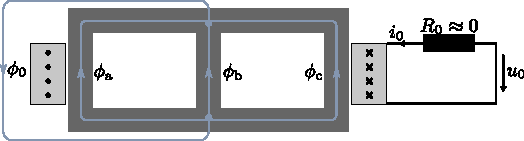
\includegraphics[width=0.7\textwidth]{fig/lec04/Zero_flux_model.pdf}
		\caption{Substitute model to represent the zero flux component}
		\label{fig:Zero_flux_model}
	\end{figure}
\end{frame}


%%%%%%%%%%%%%%%%%%%%%%%%%%%%%%%%%%%%%%%%%%%%%%%%%%%%%%%%%%%%%
%% Three-phase transformer connection and winding types %%
%%%%%%%%%%%%%%%%%%%%%%%%%%%%%%%%%%%%%%%%%%%%%%%%%%%%%%%%%%%%%
\begin{frame}
	\frametitle{Three-phase transformer connection and winding types}
		Each side of a three-phase transformer can be connected in:
		\begin{equation*}
			\mbox{Y/y: star connection,}\quad \mbox{D/d: delta connection,}\quad \mbox{Z/z: zigzag connection.}
		\end{equation*} \pause
		The winding nomenclature is as follows:
		\begin{itemize}
			\item First upper case letter: primary side (high voltage) \pause
			\item Second lower case letter: secondary side (low voltage) \pause
			\item Number ($0\ldots 11$): phase deviation between the primary and secondary side in $^\circ 30$ steps \pause
			\item Optional: N/n for neutral connection of  high/low side.
		\end{itemize}
		\begin{figure}
			\onslide<1->
			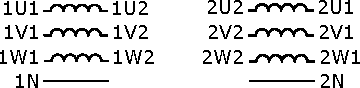
\includegraphics[width=0.45\textwidth]{fig/lec04/Connection_nomenclature_three_phase_transformer.pdf}
			\caption{Connection nomenclature of three-phase transformers}
			\label{fig:Connection_nomenclature_three_phase_transformer}
		\end{figure}
\end{frame}

%%%%%%%%%%%%%%%%%%%%%%%%%%%%%%%%%%%%%%%%%%%%%%%%%%%%%%%%%%%%%
%% Three-phase transformer connection and winding types (example: Yd1)%%
%%%%%%%%%%%%%%%%%%%%%%%%%%%%%%%%%%%%%%%%%%%%%%%%%%%%%%%%%%%%%
\begin{frame}
	\frametitle{Three-phase transformer connection and winding types (example: Yd1)}
	Transformer connection Yd1 indicates
	\begin{itemize}
		\item Y: star connection on the primary side,
		\item d: delta connection on the secondary side,
		\item 1: phase deviation of $1\cdot30^\circ=30^\circ$ between the primary and secondary side.
	\end{itemize}
	\vspace{2em}
	\begin{figure}
		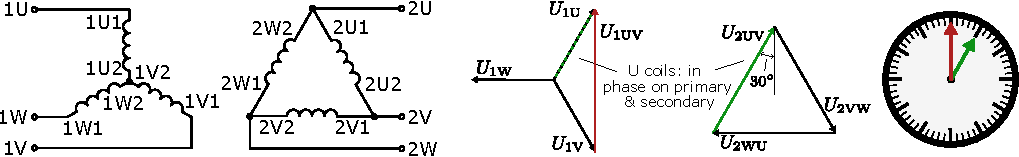
\includegraphics[width=0.99\textwidth]{fig/lec04/Yd1_example.pdf}
		\caption{Winding configuration and resulting phasor diagrams for Yd1 connection}
		\label{fig:Yd1_example}
	\end{figure}
\end{frame}

%%%%%%%%%%%%%%%%%%%%%%%%%%%%%%%%%%%%%%%%%%%%%%%%%%%%%%%%%%%%%
%% Three-phase transformer connection and winding types (example: Dy11)%%
%%%%%%%%%%%%%%%%%%%%%%%%%%%%%%%%%%%%%%%%%%%%%%%%%%%%%%%%%%%%%
\begin{frame}
	\frametitle{Three-phase transformer connection and winding types (example: Dy11)}	
	The transformer connection Dy11 indicates
	\begin{itemize}
		\item D: delta connection on the primary side,
		\item y: star connection on the secondary side,
		\item 11: phase deviation of $11\cdot30^\circ=330^\circ$ between the primary and secondary side.
	\end{itemize}
	\vspace{2em}
	\begin{figure}
		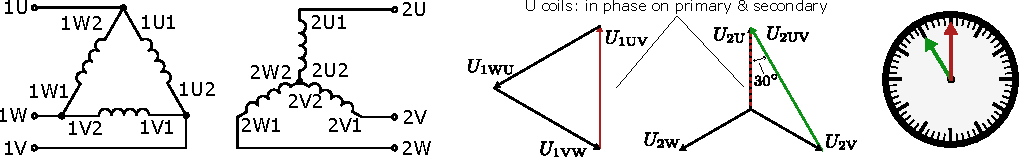
\includegraphics[width=0.99\textwidth]{fig/lec04/Dy11_example.pdf}
		\caption{Winding configuration and resulting phasor diagrams for Dy11 connection}
		\label{fig:Dy11_example}
	\end{figure}
\end{frame}

%%%%%%%%%%%%%%%%%%%%%%%%%%%%%%%%%%%%%%%%%%%%%%%%%%%%%%%%%%%%%
%% Three-phase transformer connection and winding types (example: Dy5)%%
%%%%%%%%%%%%%%%%%%%%%%%%%%%%%%%%%%%%%%%%%%%%%%%%%%%%%%%%%%%%%
\begin{frame}
	\frametitle{Three-phase transformer connection and winding types (example: Dy5)}
	In this example, the primary and secondary side are still connected in a delta-star configuration, but, the polarity of the secondary side is reversed compared to the previous Dy11 connection. Consequently, the phase deviation is $5\cdot30^\circ=150^\circ$.
	\vspace{2em}
	\begin{figure}
		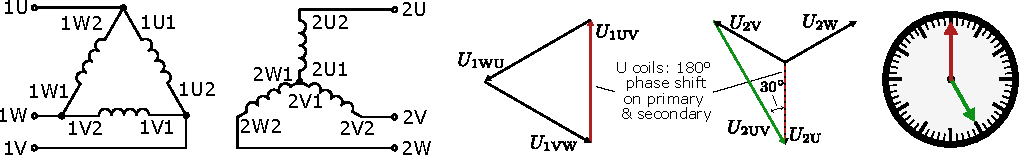
\includegraphics[width=0.99\textwidth]{fig/lec04/Dy5_example.pdf}
		\caption{Winding configuration and resulting phasor diagrams for Dy5 connection}
		\label{fig:Dy5_example}
	\end{figure}
\end{frame}


%%%%%%%%%%%%%%%%%%%%%%%%%%%%%%%%%%%%%%%%%%%%%%%%%%%%%%%%%%%%%
%% Three-phase transformer connection symbols (vector groups) %%
%%%%%%%%%%%%%%%%%%%%%%%%%%%%%%%%%%%%%%%%%%%%%%%%%%%%%%%%%%%%%
\begin{frame}
	\frametitle{Three-phase transformer connection symbols (vector groups)}
	\vspace{-0.1cm}
	\begin{figure}
		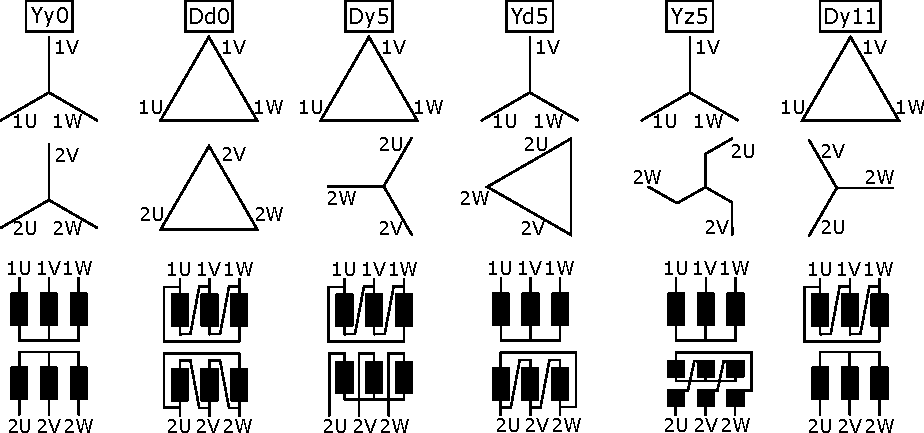
\includegraphics[height=0.75\textheight]{fig/lec04/Three_phase_transformer_connection_symbols_01.pdf}
		\caption{Exemplary (simplified) connection symbols for three-phase transformers and the resulting phasor displacement representations}
		\label{fig:Three_phase_transformer_connection_symbols_01}
	\end{figure}
\end{frame}

%%%%%%%%%%%%%%%%%%%%%%%%%%%%%%%%%%%%%%%%%%%%%%%%%%%%%%%%%%%%%
%% Three-phase transformer voltage ratio %%
%%%%%%%%%%%%%%%%%%%%%%%%%%%%%%%%%%%%%%%%%%%%%%%%%%%%%%%%%%%%%
\begin{frame}
	\frametitle{Three-phase transformer voltage ratio}
	If the three-phase connection type changes between the primary and secondary side, the voltage ratio between the primary and secondary side is affected -- cf. \tabref{tab:Three_phase_transformer_voltage_ratio}.
	\begin{table}
		\centering
		\begin{tabular}{l c c c c c c}
			\toprule
			primary & Y & D & Y & D & Y & D \\
			secondary & y & y & d & d & z & z \\
			\midrule
			$U_{1,\mathrm{ll}}/U_{2,\mathrm{ll}}$ & $1$ & $\sqrt{3}$ & $1/\sqrt{3}$ & $1$ & $\sqrt{3}/2$ & $3/2$ \\ 
			\bottomrule
		\end{tabular}
		\caption{Idealized voltage ratios between primary and secondary due to different connection types (assuming $N_1 = N_2$) with $U_{1,\mathrm{ll}}$ and $U_{2,\mathrm{ll}}$ being the line-to-line voltages on the primary and secondary side, respectively}
		\label{tab:Three_phase_transformer_voltage_ratio}
	\end{table}
\end{frame}

%%%%%%%%%%%%%%%%%%%%%%%%%%%%%%%%%%%%%%%%%%%%%%%%%%%%%%%%%%%%%
%% Dynamic modeling of the three-phase transformer %%
%%%%%%%%%%%%%%%%%%%%%%%%%%%%%%%%%%%%%%%%%%%%%%%%%%%%%%%%%%%%%
\begin{frame}
	\frametitle{Dynamic modeling of the three-phase transformer}
	Assuming a three-phase transformer without mutual coupling between the phases abc (as in the three independent single-phase transformers from \figref{fig:Three_phase_transformer_simple}) and without saturation, the magnetic flux linkage of the primary and secondary side can be expressed as
		\begin{equation}
			\bm{\psi}(t) = \begin{bmatrix} \psi_{1\mathrm{a}}(t) \\ \psi_{1\mathrm{b}}(t) \\ \psi_{1\mathrm{c}}(t) \\ \psi_{2\mathrm{a}}(t) \\ \psi_{2\mathrm{b}}(t) \\ \psi_{2\mathrm{c}}(t)\end{bmatrix} = \begin{bmatrix} L_{1\mathrm{a}} & 0 & 0 & M_{\mathrm{a}} & 0 & 0 \\ 0 & L_{1\mathrm{b}} & 0 & 0 & M_{\mathrm{b}} & 0 \\ 0 & 0 & L_{1\mathrm{c}} & 0 & 0 &M_{\mathrm{c}} \\ M_{\mathrm{a}} & 0 & 0 & L_{2\mathrm{a}} & 0 &0 \\ 0 & M_{\mathrm{b}} & 0 & 0 & L_{2\mathrm{b}} & 0 \\ 0 & 0 & M_{\mathrm{c}} & 0 & 0 &L_{2\mathrm{c}}\end{bmatrix} \begin{bmatrix} i_{1\mathrm{a}}(t) \\ i_{1\mathrm{b}}(t) \\ i_{1\mathrm{c}}(t) \\ i_{2\mathrm{a}}(t) \\ i_{2\mathrm{b}}(t) \\ i_{2\mathrm{c}}(t)\end{bmatrix} = \bm{L}\bm{i}(t).
		\end{equation}
		\pause
		If the transformer's magnetic three-phase circuit is ideally symmetric, also
		$$ M = M_{\mathrm{a}} = M_{\mathrm{b}} = M_{\mathrm{c}}, \quad L_1 = L_{1\mathrm{a}} = L_{1\mathrm{b}} = L_{1\mathrm{c}}, \quad L_2 = L_{2\mathrm{a}} = L_{2\mathrm{b}} = L_{2\mathrm{c}}$$
		holds. 
\end{frame}

%%%%%%%%%%%%%%%%%%%%%%%%%%%%%%%%%%%%%%%%%%%%%%%%%%%%%%%%%%%%%%
%%% Dynamic modeling of the three-phase transformer %%
%%%%%%%%%%%%%%%%%%%%%%%%%%%%%%%%%%%%%%%%%%%%%%%%%%%%%%%%%%%%%%
%\begin{frame}
%	\frametitle{Dynamic modeling of the three-phase transformer (cont.)}
%	Hence, we have
%		\begin{equation}
%			\bm{\psi}(t) = \begin{bmatrix} \psi_{1\mathrm{a}}(t) \\ \psi_{1\mathrm{b}}(t) \\ \psi_{1\mathrm{c}}(t) \\ \psi_{2\mathrm{a}}(t) \\ \psi_{2\mathrm{b}}(t) \\ \psi_{2\mathrm{c}}(t)\end{bmatrix} = \begin{bmatrix} L_{1} & 0 & 0 & M & 0 & 0 \\ 0 & L_{1} & 0 & 0 & M & 0 \\ 0 & 0 & L_{1} & 0 & 0 & M \\ M & 0 & 0 & L_{2} & 0 &0 \\ 0 & M & 0 & 0 & L_{2} & 0 \\ 0 & 0 & M & 0 & 0 &L_{2}\end{bmatrix} \begin{bmatrix} i_{1\mathrm{a}}(t) \\ i_{1\mathrm{b}}(t) \\ i_{1\mathrm{c}}(t) \\ i_{2\mathrm{a}}(t) \\ i_{2\mathrm{b}}(t) \\ i_{2\mathrm{c}}(t)\end{bmatrix} = \bm{L}\bm{i}(t).
%			\label{eq:Three_phase_transformer_flux_linkage}
%		\end{equation}
%		\pause
%		The voltage equation results from Faraday's law and Ohm's law:
%		\begin{equation}
%			\bm{u}(t) = \bm{R}\bm{i}(t)+ \bm{L}\frac{\mathrm{d}}{\mathrm{d}t}\bm{i}(t) = \begin{bmatrix} R_{1} & 0 & 0 & 0 & 0 & 0 \\ 0 & R_{1} & 0 & 0 & 0 & 0 \\ 0 & 0 & R_{1} & 0 & 0 & 0 \\ 0 & 0 & 0 & R_{2} & 0 &0 \\ 0 & 0 & 0 & 0 & R_{2} & 0 \\ 0 & 0 & 0 & 0 & 0 &R_{2}\end{bmatrix}\bm{i}(t)+ \bm{L}\frac{\mathrm{d}}{\mathrm{d}t}\bm{i}(t).
%		\end{equation}
%\end{frame}
%
%%%%%%%%%%%%%%%%%%%%%%%%%%%%%%%%%%%%%%%%%%%%%%%%%%%%%%%%%%%%%%
%%% Dynamic modeling of the three-phase transformer %%
%%%%%%%%%%%%%%%%%%%%%%%%%%%%%%%%%%%%%%%%%%%%%%%%%%%%%%%%%%%%%%
%\begin{frame}
%	\frametitle{Dynamic modeling of the three-phase transformer (cont.)}
%	Due to the ideal three-phase symmetry, the model relation per phase pair on the primary and secondary side are identical for all three phases, i.e., we can split up the model into:  
%	\begin{align}
%		\begin{bmatrix}	u_\mathrm{1a}(t)\\u_\mathrm{2a}(t) \end{bmatrix} &= \begin{bmatrix} R_1 & 0 \\ 0 & R_2 \end{bmatrix} \begin{bmatrix} i_\mathrm{1a}(t)\\i_\mathrm{2a}(t) \end{bmatrix} + \begin{bmatrix} L_1 & M \\ M & L_2 \end{bmatrix} \frac{\mathrm{d}}{\mathrm{d}t} \begin{bmatrix} i_\mathrm{1a}(t)\\i_\mathrm{2a}(t) \end{bmatrix}, \\   
%		\begin{bmatrix}	u_\mathrm{1b}(t)\\u_\mathrm{2b}(t) \end{bmatrix} &= \begin{bmatrix} R_1 & 0 \\ 0 & R_2 \end{bmatrix} \begin{bmatrix} i_\mathrm{1b}(t)\\i_\mathrm{2b}(t) \end{bmatrix} + \begin{bmatrix} L_1 & M \\ M & L_2 \end{bmatrix} \frac{\mathrm{d}}{\mathrm{d}t} \begin{bmatrix} i_\mathrm{1b}(t)\\i_\mathrm{2b}(t) \end{bmatrix},\\
%		\begin{bmatrix}	u_\mathrm{1c}(t)\\u_\mathrm{2c}(t) \end{bmatrix} &= \begin{bmatrix} R_1 & 0 \\ 0 & R_2 \end{bmatrix} \begin{bmatrix} i_\mathrm{1c}(t)\\i_\mathrm{2c}(t) \end{bmatrix} + \begin{bmatrix} L_1 & M \\ M & L_2 \end{bmatrix} \frac{\mathrm{d}}{\mathrm{d}t} \begin{bmatrix} i_\mathrm{1c}(t)\\i_\mathrm{2c}(t) \end{bmatrix}.
%	\end{align}
%	\pause
%	Hence, under the made assumptions the same ECD from \figref{fig:Transformer_T_ECD} for the single-phase transformer case can be also used to model the three-phase transformer.
%	\begin{figure}
%		\centering
%		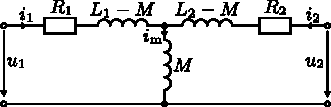
\includegraphics[width=0.38\textwidth]{fig/lec04/Transformer_T_ECD.pdf}
%	\end{figure}
%\end{frame} 